\documentclass[a4paper]{book}


% tilføjet af Stubman 231010
\usepackage[footnote,draft,danish,silent,nomargin]{fixme}		% Indst rettelser og lignende med \fixme{...} Med final i stedet for draft, udlses en error 																															for hver fixme, der ikke er slettet, nr rapporten bygges.

%%%%%%%%%% Various Packages %%%%%%%%%
\usepackage[english]{babel}
\usepackage[utf8]{inputenc}
\usepackage[numbers]{natbib}
\usepackage{verbatim}%% For Comment enviroment
%\usepackage{listings}

\usepackage{lastpage}% gives lastpage commando
\usepackage{algorithm}%%% Algorithm Eviroment
\usepackage{algorithmic}%%% Algorithm Eviroment
\usepackage{amsmath, amsfonts, amssymb, amsthm,mathtools} % Math Paths
\usepackage{bm}
\usepackage{fancyhdr} % For headers
\usepackage{sadlist} % Selfdefined package. Gives \begin{sadlist}{title}{description}{label}
\usepackage{casecontrol}%
\usepackage{packages/maplestd2e}%
\usepackage{xifthen}% provides \isempty test and ifthen else 
\usepackage[absolute]{textpos} %used on the frontpage for the picture.
\usepackage{tabularx}
\usepackage[retainorgcmds]{IEEEtrantools}
\usepackage{qtree}
\usepackage{stmaryrd}
\usepackage{morefloats}
\usepackage{placeins} % Gives the \FloatBarrier command
\usepackage{pdfpages}
\usepackage{rotating}

%%%%%%%%%%%% Words %%%%%%%%%%%%%%
\newcommand{\elearning}[1][]{\caseControl{e}{-learning}{#1}{}}%



%%%%%%%%%%%%%%%%%%%%%%%%%%%%%%

%%%%%%% Protect against orhpans and widows %%%%%%%%%
\widowpenalty=300
\clubpenalty=300
%%%%%%%%%%%%%%%%%%%%%%%%%%%%%%%



%%%%%% Depracted  %%%%%%%%
%\usepackage{en-bib}  % anyone who knows this?
%\usepackage{en-bib}  % anyone who knows this?
%%%%%%%%%%%%%%%%%%%%


%%%%%%%%% Make links work %%%%%%%%%%
\usepackage[pdfborder={0 0 0 0}, backref=none]{hyperref}
%\usepackage[a4paper, bookmarks=true, bookmarksopen=true, bookmarksnumbered=true, pdfborder={0 0 0 0}, colorlinks=true, breaklinks=true, backref=section]{hyperref}
\hypersetup{
pdfborder=0 0 0
}
%%%%%%%%%%%%%%%%%%%%%%%%%%%%%%


%%% something? useful? hopefully!
%\usepackage[]{graphicx} %dvips
\usepackage{graphicx}
%\usepackage{caption}
\usepackage{subcaption}
\usepackage{emp}
\usepackage{sidecap}
%\ifx\pdftexversion\undefined
%\usepackage[dvips]{graphicx}
%\else
%\usepackage[pdftex]{graphicx}
%\DeclareGraphicsRule{*}{mps}{*}{}
%\fi
%\usepackage[]{subfig}% Need to make several pictures in one float
\usepackage{wrapfig}% Enables us to wrap text around a figure
%%%%%%%%%%%%%%%%%%%%%%%%%%%%%


%%%%%% Prettier chapters %%%%%
%\usepackage[Lenny]{fncychap}%
%\usepackage[Sonny]{fncychap}%
%\usepackage[Glenn]{fncychap}%
%\usepackage[Bjarne]{fncychap}%
%\usepackage[Bjornstrup]{fncychap}%
%\usepackage[Conny]{fncychap}%
%\usepackage[Rejne]{fncychap}%
\usepackage{xparse}%
%%%%%%%%%%%%%%%%%%%%



%\setcitestyle{numbers}

%%%% Bibliography %%%%%%
\bibliographystyle{plainnat}
%%%%%%%%%%%%%%%%%


%%%%%% Something something might be important  %%%%%%%%%
\setcounter{secnumdepth}{3}
\setcounter{tocdepth}{2}
\linespread{1}
%%%%%%%%%%%%%%%%%%%%

%%%%%%%%% Depracted %%%%%%%%%%%
%\setlength{\marginparwidth}{10pt}
%\setlength{\textwidth}{400pt}
%\setlength{\textheight}{620pt}
%\setlength{\voffset}{0pt}
%\setlength{\hoffset}{0pt}
%\setlength{\topmargin}{0pt}
%\setlength{\headsep}{10pt}
%\setlength{\oddsidemargin}{50pt}
%\setlength{\evensidemargin}{10pt}
%%%%%%%%%%%%%%%%%%%%



%%%%%%%%%%%%  COMMANDS   %%%%%%%%%%%%%%%%%%
%%%%%%%%%%%%%%%%%%%%%%%%%%%%%%%%%%%%%%%%%%%
%%%%%%%%%%%%%%%%%%%%%%%%%%%%%%%%%%%%%%%%%%%
%%%%%%%%%%%%%%%%%%%%%%%%%%%%%%%%%%%%%%%%%%%

%%%%%%%%%% Get commands defined Elsewhere %%%%%%%%%
%% c = first letter capital
% cap = all capital
% i = italic
% b = bold
% ci = first letter cap and all italic.
 \newcommand{\theWord}{some}
\newcommand{\caseControl}[4]{%
     \ifthenelse{\equal{#3}{c}}% First letter capital
    {\renewcommand{\theWord}{\MakeUppercase{#1}#2}}% if #1 true
    {}% if #1 false
     \ifthenelse{\equal{#3}{ci}}% first letter cap and italic
    {\renewcommand{\theWord}{\textit{\MakeUppercase{#1}#2}}}% if #1 true
    {}% if #1 false
      \ifthenelse{\equal{#3}{ic}}%% first letter cap and italic
    {\renewcommand{\theWord}{\textit{\MakeUppercase{#1}#2}}}% if #1 true
    {}% if #1 false
      \ifthenelse{\equal{#3}{cb}}%% first letter cap and italic
    {\renewcommand{\theWord}{\textbf{\MakeUppercase{#1}#2}}}% if #1 true
    {}% if #1 false
        \ifthenelse{\equal{#3}{bc}}%% first letter cap and italic
    {\renewcommand{\theWord}{\textbf{\MakeUppercase{#1}#2}}}% if #1 true
    {}% if #1 false
   \ifthenelse{\equal{#3}{cbi}}%% first letter cap and italic
    {\renewcommand{\theWord}{\textbf{\MakeUppercase{#1}#2}}}% if #1 true
    {}% if #1 false
        \ifthenelse{\equal{#3}{bci}}%% first letter cap and italic
    {\renewcommand{\theWord}{\textbf{\MakeUppercase{#1}#2}}}% if #1 true
    {}% if #1 false
   \ifthenelse{\equal{#3}{icb}}%% first letter cap and italic
    {\renewcommand{\theWord}{\textbf{\MakeUppercase{#1}#2}}}% if #1 true
    {}% if #1 false
        \ifthenelse{\equal{#3}{ibc}}%% first letter cap and italic
    {\renewcommand{\theWord}{\textbf{\MakeUppercase{#1}#2}}}% if #1 true
    {}% if #1 false
   \ifthenelse{\equal{#3}{cib}}%% first letter cap and italic
    {\renewcommand{\theWord}{\textbf{\MakeUppercase{#1}#2}}}% if #1 true
    {}% if #1 false
        \ifthenelse{\equal{#3}{bic}}%% first letter cap and italic
    {\renewcommand{\theWord}{\textbf{\MakeUppercase{#1}#2}}}% if #1 true
    {}% if #1 false
   \ifthenelse{\equal{#3}{u}}%% first letter cap and italic
    {\renewcommand{\theWord}{\textbf{\MakeUppercase{#1}#2}}}% if #1 true
    {}% if #1 false
        \ifthenelse{\equal{#3}{ub}}%% first letter cap and italic
    {\renewcommand{\theWord}{\textbf{\MakeUppercase{#1}#2}}}% if #1 true
    {}% if #1 false
   \ifthenelse{\equal{#3}{bu}}%% first letter cap and italic
    {\renewcommand{\theWord}{\textbf{\MakeUppercase{#1}#2}}}% if #1 true
    {}% if #1 false
        \ifthenelse{\equal{#3}{biu}}%% first letter cap and italic
    {\renewcommand{\theWord}{\textbf{\MakeUppercase{#1}#2}}}% if #1 true
    {}% if #1 false
      \ifthenelse{\equal{#3}{i}}%% italic
    {\renewcommand{\theWord}{\textit{#1#2}}}% if #1 true
    {}% if #1 false
      \ifthenelse{\equal{#3}{b}}%% bold
    {\renewcommand{\theWord}{\textbf{#1#2}}}% if #1 true
    {}% if #1 false
     \ifthenelse{\equal{#3}{cap}}% all cap
    {\renewcommand{\theWord}{\MakeUppercase{#1#2}}}% if #1 true
    {}% if #1 false
       \ifthenelse{\isempty{#3}}% %if nothing is stated 
    {\renewcommand{\theWord}{#1#2}}% if #1 true
    {}% if #1 false 
    \ifthenelse{\equal{\theWord}{some}}% % Double check actually
    {\renewcommand{\theWord}{#1#2 }}% if #1 true
    {}% if #1 false 
    %%%%%% Standard definitions of words %%%%%%
        \ifthenelse{\equal{#4}{i}}% 
    {\textit{\theWord}}% if #1 true  % Print it italic
    {}% if #1 false 
	    \ifthenelse{\equal{#4}{b}}% Print it in bold
    {\textbf{\theWord}}% if #1 true
    {}% if #1 false 
        \ifthenelse{\equal{#4}{u}}% print it underlinde (not working yet)
    {{\theWord}}% if #1 true
    {}% if #1 false 
       \ifthenelse{\isempty{#4}}%  If there is nothing stated here just print the shit. 
    {\theWord}% if #1 true
    {}% if #1 false    
    \renewcommand{\theWord}{some}%
  }
\newcommand{\myMonth}{Some}
\newcommand{\myDate}[3]{%
\ifthenelse{\equal{#2}{1}}%
{\renewcommand{\myMonth}{January}}{}%
\ifthenelse{\equal{#2}{2}}%
{\renewcommand{\myMonth}{February}}{}%
\ifthenelse{\equal{#2}{3}}%
{\renewcommand{\myMonth}{Marts}}{}%
\ifthenelse{\equal{#2}{4}}%
{\renewcommand{\myMonth}{April}}{}%
\ifthenelse{\equal{#2}{5}}%
{\renewcommand{\myMonth}{May}}{}%
\ifthenelse{\equal{#2}{6}}%
{\renewcommand{\myMonth}{June}}{}%
\ifthenelse{\equal{#2}{7}}%
{\renewcommand{\myMonth}{July}}{}%
\ifthenelse{\equal{#2}{8}}%
{\renewcommand{\myMonth}{August}}{}%
\ifthenelse{\equal{#2}{9}}%
{\renewcommand{\myMonth}{September}}{}%
\ifthenelse{\equal{#2}{10}}%    
{\renewcommand{\myMonth}{October}}{}%
\ifthenelse{\equal{#2}{11}}%
{\renewcommand{\myMonth}{November}}{}%
\ifthenelse{\equal{#2}{12}}%
{\renewcommand{\myMonth}{December}}{}%
\ifthenelse{\isempty{#1}}%
{\myMonth{} #3}%
{\myMonth{} #1, #3}}%
%% This is where we define words. 
%% The last parameter should be blank as standard, but you can add i,b,u. 

%% WORD LIST
%% This is where we define words. 
%% The last parameter should be blank as standard, but you can add i,b,u. 


\newcommand{\admpers}[1][]{\caseControl{a}{dministrative personnel}{#1}{}}%

\newcommand{\block}[1][]{\caseControl{M}{oodle block}{#1}{}}%
\newcommand{\groupname}{Project Group Team}
\newcommand{\systemname}[1][]{\caseControl{M}{yMoodle}{#1}{}}%
\newcommand{\admlib}[1][]{\caseControl{a}{dmin tool library}{#1}{}}%
\newcommand{\subsystem}[1][]{\caseControl{s}{ub-system}{#1}{}}%
\newcommand{\subgroup}[1][]{\caseControl{s}{ub-group}{#1}{}}%
\newcommand{\sn}[1][]{\systemname[]}
\newcommand{\systemmode}[1][]{\caseControl{``F}{ollow mode''}{#1}{}}%
\newcommand{\sm}[1][]{\systemmode[#1]}%
\newcommand{\viewroom}[1][]{\caseControl{v}{iew}{#1}{}}%

%car names
\newcommand{\leader}[1][]{\caseControl{S}{pinky}{#1}{}}%
\newcommand{\follower}[1][]{\caseControl{T}{he Dutch Rammer}{#1}{}}%


\newcommand{\rdesc}[1][]{\caseControl{r}{ecursive-descent}{#1}{}}%
\newcommand{\mas}[1][]{\caseControl{m}{ulti agent system}{#1}{}}%
\newcommand{\idt}[1][]{\caseControl{i}{dentification table}{#1}{}}%
\newcommand{\agd}[1][]{\caseControl{A}{rongadongk}{#1}{}}%
\newcommand{\abst}[1][]{\caseControl{a}{bstract syntax tree}{#1}{}}%

\newcommand{\ooad}[1][]{OOAD}%
\newcommand{\ainterface}[1][]{\caseControl{A}{dmin Interface}{#1}{}}%
\newcommand{\cinterface}[1][]{\caseControl{C}{lient Interface}{#1}{}}%
\newcommand{\sinterface}[1][]{\caseControl{S}{taff Interface}{#1}{}}%
\newcommand{\helpdesk}[1][]{\caseControl{H}{opla Helpdesk}{#1}{}}%
\newcommand{\hdesk}[1][]{\caseControl{H}{opla Helpdesk}{#1}{}}
%\newcommand{\wmon}[1][]{\caseControl{w}{orkload monitor}{#1}{}}
\newcommand{\staff}[1][]{\caseControl{s}{taff}{#1}{}}
\newcommand{\client}[1][]{\caseControl{c}{lient}{#1}{}{}}%
\newcommand{\astaff}[1][]{\caseControl{s}{taff}{#1}{}}
\newcommand{\aclient}[1][]{\caseControl{c}{lient}{#1}{}{}}%
\newcommand{\sadmin}[1][]{\caseControl{a}{dmin}{#1}{}}
\newcommand{\admin}[1][]{\caseControl{a}{dmin}{#1}{}}
\newcommand{\ucsproblem}[1][]{\caseControl{s}{ubmit problem}{#1}{}}
\newcommand{\ucsolproblem}[1][]{\caseControl{s}{olve problem}{#1}{}}
\newcommand{\closed}[1][]{\caseControl{c}{losed}{#1}{}}
\newcommand{\open}[1][]{\caseControl{u}{nsolved}{#1}{}}
\newcommand{\solved}[1][]{\caseControl{s}{olved}{#1}{}}
\newcommand{\unsolved}[1][]{\caseControl{a}{ctive}{#1}{}}
\newcommand{\pinactive}[1][]{\caseControl{c}{losed}{#1}{}}
\newcommand{\pactive}[1][]{\caseControl{a}{ctive}{#1}{}}
\newcommand{\gstat}[1][]{\caseControl{s}{tatistics}{#1}{}}
\newcommand{\bloadwork}[1][]{\caseControl{b}{alance loadwork}{#1}{}}
\newcommand{\worklist}[1][]{\caseControl{w}{orklist}{#1}{}}
\newcommand{\todolist}[1][]{\caseControl{w}{orklist}{#1}{}}
\newcommand{\problem}[1][]{\caseControl{p}{roblem}{#1}{}}
\newcommand{\tucadmin}[1][]{\caseControl{a}{dministrate}{#1}{}}
\newcommand{\sql}[1][]{SQL} % just in case...
\newcommand{\aspnet}[1][]{ASP.NET} % just in case...
\newcommand{\posgresql}[1][]{PostgreSQL}
\newcommand{\iis}[1][]{IIS}
\newcommand{\wholeiis}[1][]{Microsoft Internet Information Services}
\newcommand{\spinterface}[1]{\caseControl{s}{olve admin interface}{#1}{}}
\newcommand{\viewmodel}[1]{\caseControl{v}{iew model}{#1}{}}


\newcommand{\Hdesk}[1][]{\hdesk[c]}
\newcommand{\Wmon}[1][]{\wmon[c]}
\newcommand{\Staff}[1][]{\staff[c]}
\newcommand{\Client}[1][]{\client[c]}
\newcommand{\Astaff}[1][]{\astaff[c]}
\newcommand{\Aclient}[1][]{\aclient[c]}
\newcommand{\Helpdesk}[1][]{\helpdesk[c]}
\newcommand{\Sadmin}[1][]{\sadmin[c]}
\newcommand{\Admin}[1][]{\admin[c]}

\newcommand{\john}[1][]{\caseControl{j}{ohn}{#1}{}}
\newcommand{\michael}[1][]{\caseControl{M}{ikael}{#1}{}}
\newcommand{\rubik}[1][]{\caseControl{R}{ubik's Cube}{#1}{}}
\newcommand{\facet}[1][]{\caseControl{f}{acelet}{#1}{}}
\newcommand{\facelet}[1][]{\caseControl{f}{acelet}{#1}{}}
\newcommand{\cube}[1][]{\caseControl{R}{ubik's Cube}{#1}{}}
\newcommand{\cuber}[1][]{\caseControl{c}{uber}{#1}{}}
\newcommand{\face}[1][]{\caseControl{f}{ace}{#1}{}}
\newcommand{\cpiece}[1][]{\caseControl{c}{ubie}{#1}{}}% Not that the one below are the same as this one
\newcommand{\cubie}[1][]{\caseControl{c}{ubie}{#1}{}}%
\newcommand{\cubicle}[1][]{\caseControl{c}{ubicle}{#1}{}}
\newcommand{\twist}[1][]{\caseControl{t}{wist}{#1}{}}
%\newcommand{\turn}[1][]{\caseControl{t}{urn}{#1}{}}
%\newcommand{\rotate}[1][]{\caseControl{r}{otate}{#1}{}}
\newcommand{\erno}[1][]{\caseControl{E}{rn\"{o} Rubik}{#1}{}}
\newcommand{\mpuzzle}[1][]{\caseControl{M}{agic Puzzle}{#1}{}}
\newcommand{\msquare}[1][]{\caseControl{M}{agic Square}{#1}{}}
\newcommand{\mcube}[1][]{\caseControl{M}{agic Cube}{#1}{}}

 

%\input{extra}
%%%%%%%%%%%%%%%%%%%%

%%%%  Makes the titles look nicer. i guess. Rasmus out. %%%%%%% Don't remove
%\usepackage{titlesec} \newcommand{\bigrule}{\titlerule[0.5mm]} \titleformat{\chapter}[display] {\bfseries\Huge} {  \vskip-2em 
 %\titlerule 
% \filright  \huge\chaptertitlename\ \vspace{5mm}  \huge\thechapter} {0mm} {\filright} [\vspace{3mm} \bigrule \vspace{-10mm}] %
%%%%%%%%%%%%%%%%%%%%%%%%%%%%

%%%%% Depracted %%%%%%%%%
\newcommand{\picturepath}[1]{input/pics/}


%%%%% Used to determine the highlight of the first word in the terminology %%%%%
\newcommand{\myTermHigh}[1]{\textbf{#1}: }
%%%%%%%%%%%%%%%%%%%%%%

%%%%%%%%% tops 'n' tails %%%%%%%%%%%%
\newcommand{\myTop}[1]{\vspace{-8mm}  \vspace{0mm} \textit{#1} \vspace{2.6mm} \hrule  \vspace{4.2mm} }

%\newcommand{\myTop}[1]{\vspace{-8mm}  \vspace{0mm} \textit{#1} \vspace{3.4mm} \hrule \vspace{3.4mm} }
%\newcommand{\myTop}[1]{ \vspace{3.4mm} \textit{#1} \  \\  \hrule \  \\}%
\newcommand{\myTail}[1]{ \vspace{3.4mm} \hrule \vspace{3.4mm} \textit{#1} }%

\newcommand{\emptyTop}[0]{\vspace{-6mm}}
%%%%%%%%%%%%%%%%%%%%%%%%%%%%

%%%%%%%%% Use this for caption text %%%%%%%%%%
\newcommand{\myCaption}[1]{\textit{\footnotesize #1.}}
\newcommand{\morscaption}[1]{\caption{\myCaption{#1}}}
%\usepackage[bf]{caption}
%%%%%%%%%%%%%%%%%%%%%%%%%%%%

%%%%%%%% Bruges til skillekolonner og r\ae{}kker . Definerer tykkelsen. %%%%%%
\newcommand{\vrules}{{\vrule width 0.6pt}}
\newcommand{\hrules}{{\hrule height 1.2pt}}
%%%%%%%%%%%%%%%%%%%%%%%%%%%%%%%%%%%%%%%%%%%

%%%%%%%Commands for getting e.g. ``st'' lifted in 1st   %%%%%%%%%%%
\newcommand{\superscript}[1]{\ensuremath{^{\textrm{#1}}}}
\newcommand{\subscript}[1]{\ensuremath{_{\textrm{#1}}}}
\newcommand{\ths}[0]{\superscript{th}}
\newcommand{\st}[0]{\superscript{st}}
\newcommand{\nd}[0]{\superscript{nd}}
\newcommand{\rd}[0]{\superscript{rd}}
%%%%%%%%%%%%%%%%%%%%%%%%%%%%%%%%%%%%%%%%%%%

%%%%%%%%% FIXME macro %%%%%%%%%%%%
%\newcommand{\todo}[1]{\fxnote{#1}}
%\newcommand{\todoV}[1]{\fxfatal{#1}}
%\newcommand{\todov}[1]{\fxfatal{#1}}

%%%%%%%%%%%%%%%%%%%%%%%%%%%%%%%%%%

%%%%%%%%% REFERENCES %%%%%%%%%%%%%
\newcommand{\agdref}[2]{#1~\ref{#2}}

%%%%%%%%%%%%%%%%%%%%%%%%%%%%%%%%%%

%%%%%%%%%% Moves %%%%%%%%%%
\newcommand{\m}[1]{\textbf{#1}}
\newcommand{\vr}[1]{$#1$}
\newcommand{\pcparagraph}[1]{\vspace{-1.5mm}\paragraph{#1}}
%%%%%%%%%%%%

%%%%%%%%%%%%%%%%%%%%%%%%%%%


\newcommand{\OK}[0]{\textsc{Ok}}
\newcommand{\Ok}[0]{\textsc{Ok}}
\newcommand{\Undef}[0]{\textsc{Undefined}}
\newcommand{\Wrong}[0]{\textsc{Wrong}}
\newcommand{\Nil}[0]{\textsc{Nil}}
\newcommand{\sensorDist}[0]{15 cm}

%%%%%%%%%%%%%%%%%%%%%%%%%%%%%%%%
% JOURNALS %%
\newcommand{\journalwidth}[0]{\textwidth}


%%%%%%%%%%%%%%%%%%%%%%%%%%%

%%%%%%%%%% Class, component ... %%%%%%%%%%%%%%%%%%

\newcommand{\me}[1]{\method{#1}}							%%Don't change
\newcommand{\class}[1]{\textbf{#1}}						%%Do change
\newcommand{\cl}[1]{\class{#1}}								%%Don't change
\newcommand{\aclass}[1]{\textit{\class{#1}}}	%%Do change
\newcommand{\acl}[1]{\aclass{#1}}							%%Don't change
\newcommand{\component}[1]{\textbt{#1}}				%%Do change
\newcommand{\comp}[1]{\component{#1}}					%%Don't change
\newcommand{\vari}[1]{\mbox{\textbf{#1}}}						%%Do change
\newcommand{\method}[1]{\mbox{\texttt{#1}}}						%%Do change
\newcommand{\function}[1]{\method{#1}}				%%Do change
\newcommand{\fu}[1]{\function{#1}}						%%Don't change
\newcommand{\field}[1]{\mbox{\textbf{#1}}}						%%Do change
\newcommand{\relation}[1]{\mbox{\texttt{#1}}}						%%Do change
\newcommand{\rel}[1]{\relation{#1}}						%%Don't change
\newcommand{\requirement}[1]{#1}						%%Do change
\newcommand{\req}[1]{\requirement{#1}}						%%Don't change

\newcommand{\figref}[1]{Figure~\ref{#1}}			%%Do change
\newcommand{\coderef}[1]{Code Snippet~\ref{#1}}	%%Do change
\newcommand{\chapref}[1]{Chapter~\ref{#1}}			%%Do change
\newcommand{\secref}[1]{Section~\ref{#1}}			%%Do change
\newcommand{\partref}[1]{Part~\ref{#1}}			%%Do change
\newcommand{\appref}[1]{Appendix~\ref{#1}}			%%Do change
\newcommand{\lineref}[1]{line~\ref{#1}}			%%Do change
\newcommand{\linesref}[2]{lines~\ref{#1}-\ref{#2}}			%%Do change


\newcommand{\type}[1]{\textbf{#1}} % added by Stubman 110420
\newcommand{\object}[1]{\texttt{#1}} % added by Stubman 110420

%%%%%%%%%%%%%%%%%%%%%%%%%%%%%%%%%%%%%%%%%%%%%%%%%%

%%%%%%%%%%%%%%% Qoutations %%%%%%%%%%%%
\newcolumntype{R}{>{\raggedleft\arraybackslash}X}%
\newcommand{\myQuote}[1]{
\begin{flushleft}
\Huge{\textbf{``}}
\end{flushleft}
\vspace{-30pt}
\begin{quote}
#1
\end{quote}
\vspace{-30pt}
\begin{flushright}
\Huge{\textbf{''}}
\end{flushright}
}


%%%%%%%%% Defining Theorem %%%%%%%%%%%
\theoremstyle{definition} \newtheorem{theorem}{Theorem}
%%%%%%%%%%%%%%%%%%%%%%%%%%%%%%%%%%%%%%%%%%%

%%%%%%%%% Multi Row %%%%%%%%%%%%%%%%%%%
\usepackage{multirow}
%%% This is needed to use the multicolumn command
%%%%%%%%%%%%%%%%%%%%%%%%%%%%%%%%%%%%%%%%%%%
\hyphenation{help-desk}

%%%%%%%%%%%%%%%%%%%%%%%%%%%%%%%%%%%%%%%%%%%%%%%%
%%% Environments for operational semantics
%%%%%%%%%%%%%%%%%%%%%%%%%%%%%%%%%%%%%%%%%%%%%%%%
\newcommand{\envv}{\textit{env}_{v}}
\newcommand{\envf}{\textit{env}_{f}}
\newcommand{\sto}{\textit{sto}}
\newcommand{\ret}{\textit{ret}}
\newcommand{\Void}{\textsc{Void}}
\newcommand{\Int}{\textit{Int}}
\newcommand{\Float}{\textit{Float}}
\newcommand{\Bool}{\textit{Bool}}
\newcommand{\String}{\textit{String}}
\newcommand{\Types}{\textbf{Types}}
\newcommand{\semspace}{\vspace{-6mm}}

%%%%%%%%% List Environments %%%%%%%%%%%
\usepackage{listings}


\usepackage{color}

\definecolor{light-gray}{gray}{0.80}
\definecolor{gray95}{gray}{.95}
\definecolor{gray92}{gray}{.92}
\definecolor{gray75}{gray}{.75}
\definecolor{gray45}{gray}{.45}

\lstdefinestyle{arongadongkCode}
{ 
	%numbers=left,
	numbersep=5pt, 
	stepnumber=1,
	captionpos=b,  %bottom
	keywordstyle=\color[rgb]{0,0,1},
	commentstyle=\color[rgb]{0.133,0.545,0.133},
	stringstyle=\color[rgb]{0.627,0.126,0.941},
	%backgroundcolor=\color{gray95},
	%frame=lrtb,
	framerule=0.5pt,
	linewidth=1.00\textwidth,
	tabsize=4,
	numberbychapter=true,
	basicstyle=\ttfamily\footnotesize,
	breaklines=true,
	showstringspaces=false,
	morecomment=[l]{//},
	morecomment=[s]{/*}{*/},
	emph=[1]{int,string,float,bool},%%%%%%%%%%% Types
	emph=[2]{global,const,if,while,else,return}, %%%%%%%%%%% Keywords
	emphstyle=[1]{\color[rgb]{0,0.7,0.7}},
	emphstyle=[2]{\color[rgb]{0.7,0,1}},
	float=htb,
	breakindent=20pt
}

\lstdefinestyle{sourceCode}
{ 
	numbers=left,
	numbersep=5pt, 
	stepnumber=1,
	captionpos=b,  %bottom
	keywordstyle=\color[rgb]{0,0,1},
	commentstyle=\color[rgb]{0.133,0.545,0.133},
	stringstyle=\color[rgb]{0.627,0.126,0.941},
	%backgroundcolor=\color{gray95},
	%frame=lrtb,
	framerule=0.5pt,
	linewidth=1.00\textwidth,
	tabsize=4,
	numberbychapter=true,
	basicstyle=\ttfamily\footnotesize,
	language=C,
	breaklines=true,
	showstringspaces=false,
	emph=[1]{endregion,region,get,set,enum},%%%%%%%%%%% Add new keywords here
	%emph=[2]{Tag,Problem,Person,List,NotSupportedException,TestMethod,ProblemSearch,Assert,
	%EntityCollection,Department,IEnumerable,TimeSpan,DateTime},%%Classes
	emphstyle=[1]{\color[rgb]{0,0,1}},
	emphstyle=[1]{\color[rgb]{0,0,1}},
	emphstyle=[2]{\color[rgb]{0.1,0.5,0.5}},
	float=htb,
	breakindent=20pt
}
\lstdefinestyle{phpCode}
{ 
	numbers=left,
	numbersep=5pt, 
	stepnumber=1,
	captionpos=b,  %bottom
	keywordstyle=\color[rgb]{0,0,1},
	commentstyle=\color[rgb]{0.133,0.545,0.133},
	stringstyle=\color[rgb]{0.627,0.126,0.941},
	%backgroundcolor=\color{gray95},
	%frame=lrtb,
	framerule=0.5pt,
	linewidth=1.00\textwidth,
	tabsize=4,
	numberbychapter=true,
	basicstyle=\ttfamily\footnotesize,
	language=PHP,
	breaklines=true,
	showstringspaces=false,
	emph=[1]{class,extends,new,return,function},%%%%%%%%%%% Add new keywords here
	%emph=[2]{Tag,Problem,Person,List,NotSupportedException,TestMethod,ProblemSearch,Assert,
	%EntityCollection,Department,IEnumerable,TimeSpan,DateTime},%%Classes
	emphstyle=[1]{\color[rgb]{0,0,1}},
	emphstyle=[1]{\color[rgb]{0,0,1}},
	emphstyle=[2]{\color[rgb]{0.1,0.5,0.5}},
	float=htb,
	breakindent=20pt
}

\lstdefinestyle{oilCode}
{ 
	%numbers=left,
	numbersep=5pt, 
	stepnumber=1,
	captionpos=b,  %bottom
	keywordstyle=\color[rgb]{0,0,1},
	commentstyle=\color[rgb]{0.133,0.545,0.133},
	stringstyle=\color[rgb]{0.627,0.126,0.941},
	%backgroundcolor=\color{gray95},
	%frame=lrtb,
	framerule=0.5pt,
	linewidth=1.00\textwidth,
	tabsize=4,
	numberbychapter=true,
	basicstyle=\ttfamily\footnotesize,
	language=C,
	breaklines=true,
	showstringspaces=false,
	emph=[1]{Task},%%%%%%%%%%% Add new keywords here
	%emph=[2]{Tag,Problem,Person,List,NotSupportedException,TestMethod,ProblemSearch,Assert,
	%EntityCollection,Department,IEnumerable,TimeSpan,DateTime},%%Classes
	emphstyle=[1]{\color[rgb]{0,0,1}},
	emphstyle=[1]{\color[rgb]{0,0,1}},
	emphstyle=[2]{\color[rgb]{0.1,0.5,0.5}},
	breakindent=20pt
}

%\renewcommand{\follower}{Ju{}dge John{}son}%Asure uncorrect noname :P Bondo you DAAUGH
\renewcommand{\lstlistingname}{Code Snippet}%%Changing the caption to read ``Code snippet''
\renewcommand{\lstlistlistingname}{List of Code Snippets}
\lstset{escapeinside={(*}{*)}}%%Defines the escape and unescape chars

%%%%%%%%%% To use with copy-paste:
\begin{comment}

\begin{lstlisting}[style=sourceCode, caption=\myCaption{<some caption>}, label=<some label>]
<the code>
	<more code, now with indent>
\end{lstlisting}

\end{comment}
%%%%%%%%%% To input file:
\begin{comment}

\lstinputlisting[style=sourceCode, caption=\myCaption{<some caption>}, label=<some label>]{<file name>}

\end{comment}


\newcommand{\moodlefile}[1]{#1}
\newcommand{\sharedReport}[0]{../../sw6-mymoodle-group/shared_report/}
\input{\sharedReport preamble}
%\documentclass[a4paper]{book}


% tilføjet af Stubman 231010
\usepackage[footnote,draft,danish,silent,nomargin]{fixme}		% Indst rettelser og lignende med \fixme{...} Med final i stedet for draft, udlses en error 																															for hver fixme, der ikke er slettet, nr rapporten bygges.

%%%%%%%%%% Various Packages %%%%%%%%%
\usepackage[english]{babel}
\usepackage[utf8]{inputenc}
\usepackage[numbers]{natbib}
\usepackage{verbatim}%% For Comment enviroment
%\usepackage{listings}

\usepackage{lastpage}% gives lastpage commando
\usepackage{algorithm}%%% Algorithm Eviroment
\usepackage{algorithmic}%%% Algorithm Eviroment
\usepackage{amsmath, amsfonts, amssymb, amsthm,mathtools} % Math Paths
\usepackage{bm}
\usepackage{fancyhdr} % For headers
\usepackage{sadlist} % Selfdefined package. Gives \begin{sadlist}{title}{description}{label}
\usepackage{casecontrol}%
\usepackage{packages/maplestd2e}%
\usepackage{xifthen}% provides \isempty test and ifthen else 
\usepackage[absolute]{textpos} %used on the frontpage for the picture.
\usepackage{tabularx}
\usepackage[retainorgcmds]{IEEEtrantools}
\usepackage{qtree}
\usepackage{stmaryrd}
\usepackage{morefloats}
\usepackage{placeins} % Gives the \FloatBarrier command
\usepackage{pdfpages}
\usepackage{rotating}

%%%%%%%%%%%% Words %%%%%%%%%%%%%%
\newcommand{\elearning}[1][]{\caseControl{e}{-learning}{#1}{}}%



%%%%%%%%%%%%%%%%%%%%%%%%%%%%%%

%%%%%%% Protect against orhpans and widows %%%%%%%%%
\widowpenalty=300
\clubpenalty=300
%%%%%%%%%%%%%%%%%%%%%%%%%%%%%%%



%%%%%% Depracted  %%%%%%%%
%\usepackage{en-bib}  % anyone who knows this?
%\usepackage{en-bib}  % anyone who knows this?
%%%%%%%%%%%%%%%%%%%%


%%%%%%%%% Make links work %%%%%%%%%%
\usepackage[pdfborder={0 0 0 0}, backref=none]{hyperref}
%\usepackage[a4paper, bookmarks=true, bookmarksopen=true, bookmarksnumbered=true, pdfborder={0 0 0 0}, colorlinks=true, breaklinks=true, backref=section]{hyperref}
\hypersetup{
pdfborder=0 0 0
}
%%%%%%%%%%%%%%%%%%%%%%%%%%%%%%


%%% something? useful? hopefully!
%\usepackage[]{graphicx} %dvips
\usepackage{graphicx}
%\usepackage{caption}
\usepackage{subcaption}
\usepackage{emp}
\usepackage{sidecap}
%\ifx\pdftexversion\undefined
%\usepackage[dvips]{graphicx}
%\else
%\usepackage[pdftex]{graphicx}
%\DeclareGraphicsRule{*}{mps}{*}{}
%\fi
%\usepackage[]{subfig}% Need to make several pictures in one float
\usepackage{wrapfig}% Enables us to wrap text around a figure
%%%%%%%%%%%%%%%%%%%%%%%%%%%%%


%%%%%% Prettier chapters %%%%%
%\usepackage[Lenny]{fncychap}%
%\usepackage[Sonny]{fncychap}%
%\usepackage[Glenn]{fncychap}%
%\usepackage[Bjarne]{fncychap}%
%\usepackage[Bjornstrup]{fncychap}%
%\usepackage[Conny]{fncychap}%
%\usepackage[Rejne]{fncychap}%
\usepackage{xparse}%
%%%%%%%%%%%%%%%%%%%%



%\setcitestyle{numbers}

%%%% Bibliography %%%%%%
\bibliographystyle{plainnat}
%%%%%%%%%%%%%%%%%


%%%%%% Something something might be important  %%%%%%%%%
\setcounter{secnumdepth}{3}
\setcounter{tocdepth}{2}
\linespread{1}
%%%%%%%%%%%%%%%%%%%%

%%%%%%%%% Depracted %%%%%%%%%%%
%\setlength{\marginparwidth}{10pt}
%\setlength{\textwidth}{400pt}
%\setlength{\textheight}{620pt}
%\setlength{\voffset}{0pt}
%\setlength{\hoffset}{0pt}
%\setlength{\topmargin}{0pt}
%\setlength{\headsep}{10pt}
%\setlength{\oddsidemargin}{50pt}
%\setlength{\evensidemargin}{10pt}
%%%%%%%%%%%%%%%%%%%%



%%%%%%%%%%%%  COMMANDS   %%%%%%%%%%%%%%%%%%
%%%%%%%%%%%%%%%%%%%%%%%%%%%%%%%%%%%%%%%%%%%
%%%%%%%%%%%%%%%%%%%%%%%%%%%%%%%%%%%%%%%%%%%
%%%%%%%%%%%%%%%%%%%%%%%%%%%%%%%%%%%%%%%%%%%

%%%%%%%%%% Get commands defined Elsewhere %%%%%%%%%
%% c = first letter capital
% cap = all capital
% i = italic
% b = bold
% ci = first letter cap and all italic.
 \newcommand{\theWord}{some}
\newcommand{\caseControl}[4]{%
     \ifthenelse{\equal{#3}{c}}% First letter capital
    {\renewcommand{\theWord}{\MakeUppercase{#1}#2}}% if #1 true
    {}% if #1 false
     \ifthenelse{\equal{#3}{ci}}% first letter cap and italic
    {\renewcommand{\theWord}{\textit{\MakeUppercase{#1}#2}}}% if #1 true
    {}% if #1 false
      \ifthenelse{\equal{#3}{ic}}%% first letter cap and italic
    {\renewcommand{\theWord}{\textit{\MakeUppercase{#1}#2}}}% if #1 true
    {}% if #1 false
      \ifthenelse{\equal{#3}{cb}}%% first letter cap and italic
    {\renewcommand{\theWord}{\textbf{\MakeUppercase{#1}#2}}}% if #1 true
    {}% if #1 false
        \ifthenelse{\equal{#3}{bc}}%% first letter cap and italic
    {\renewcommand{\theWord}{\textbf{\MakeUppercase{#1}#2}}}% if #1 true
    {}% if #1 false
   \ifthenelse{\equal{#3}{cbi}}%% first letter cap and italic
    {\renewcommand{\theWord}{\textbf{\MakeUppercase{#1}#2}}}% if #1 true
    {}% if #1 false
        \ifthenelse{\equal{#3}{bci}}%% first letter cap and italic
    {\renewcommand{\theWord}{\textbf{\MakeUppercase{#1}#2}}}% if #1 true
    {}% if #1 false
   \ifthenelse{\equal{#3}{icb}}%% first letter cap and italic
    {\renewcommand{\theWord}{\textbf{\MakeUppercase{#1}#2}}}% if #1 true
    {}% if #1 false
        \ifthenelse{\equal{#3}{ibc}}%% first letter cap and italic
    {\renewcommand{\theWord}{\textbf{\MakeUppercase{#1}#2}}}% if #1 true
    {}% if #1 false
   \ifthenelse{\equal{#3}{cib}}%% first letter cap and italic
    {\renewcommand{\theWord}{\textbf{\MakeUppercase{#1}#2}}}% if #1 true
    {}% if #1 false
        \ifthenelse{\equal{#3}{bic}}%% first letter cap and italic
    {\renewcommand{\theWord}{\textbf{\MakeUppercase{#1}#2}}}% if #1 true
    {}% if #1 false
   \ifthenelse{\equal{#3}{u}}%% first letter cap and italic
    {\renewcommand{\theWord}{\textbf{\MakeUppercase{#1}#2}}}% if #1 true
    {}% if #1 false
        \ifthenelse{\equal{#3}{ub}}%% first letter cap and italic
    {\renewcommand{\theWord}{\textbf{\MakeUppercase{#1}#2}}}% if #1 true
    {}% if #1 false
   \ifthenelse{\equal{#3}{bu}}%% first letter cap and italic
    {\renewcommand{\theWord}{\textbf{\MakeUppercase{#1}#2}}}% if #1 true
    {}% if #1 false
        \ifthenelse{\equal{#3}{biu}}%% first letter cap and italic
    {\renewcommand{\theWord}{\textbf{\MakeUppercase{#1}#2}}}% if #1 true
    {}% if #1 false
      \ifthenelse{\equal{#3}{i}}%% italic
    {\renewcommand{\theWord}{\textit{#1#2}}}% if #1 true
    {}% if #1 false
      \ifthenelse{\equal{#3}{b}}%% bold
    {\renewcommand{\theWord}{\textbf{#1#2}}}% if #1 true
    {}% if #1 false
     \ifthenelse{\equal{#3}{cap}}% all cap
    {\renewcommand{\theWord}{\MakeUppercase{#1#2}}}% if #1 true
    {}% if #1 false
       \ifthenelse{\isempty{#3}}% %if nothing is stated 
    {\renewcommand{\theWord}{#1#2}}% if #1 true
    {}% if #1 false 
    \ifthenelse{\equal{\theWord}{some}}% % Double check actually
    {\renewcommand{\theWord}{#1#2 }}% if #1 true
    {}% if #1 false 
    %%%%%% Standard definitions of words %%%%%%
        \ifthenelse{\equal{#4}{i}}% 
    {\textit{\theWord}}% if #1 true  % Print it italic
    {}% if #1 false 
	    \ifthenelse{\equal{#4}{b}}% Print it in bold
    {\textbf{\theWord}}% if #1 true
    {}% if #1 false 
        \ifthenelse{\equal{#4}{u}}% print it underlinde (not working yet)
    {{\theWord}}% if #1 true
    {}% if #1 false 
       \ifthenelse{\isempty{#4}}%  If there is nothing stated here just print the shit. 
    {\theWord}% if #1 true
    {}% if #1 false    
    \renewcommand{\theWord}{some}%
  }
\newcommand{\myMonth}{Some}
\newcommand{\myDate}[3]{%
\ifthenelse{\equal{#2}{1}}%
{\renewcommand{\myMonth}{January}}{}%
\ifthenelse{\equal{#2}{2}}%
{\renewcommand{\myMonth}{February}}{}%
\ifthenelse{\equal{#2}{3}}%
{\renewcommand{\myMonth}{Marts}}{}%
\ifthenelse{\equal{#2}{4}}%
{\renewcommand{\myMonth}{April}}{}%
\ifthenelse{\equal{#2}{5}}%
{\renewcommand{\myMonth}{May}}{}%
\ifthenelse{\equal{#2}{6}}%
{\renewcommand{\myMonth}{June}}{}%
\ifthenelse{\equal{#2}{7}}%
{\renewcommand{\myMonth}{July}}{}%
\ifthenelse{\equal{#2}{8}}%
{\renewcommand{\myMonth}{August}}{}%
\ifthenelse{\equal{#2}{9}}%
{\renewcommand{\myMonth}{September}}{}%
\ifthenelse{\equal{#2}{10}}%    
{\renewcommand{\myMonth}{October}}{}%
\ifthenelse{\equal{#2}{11}}%
{\renewcommand{\myMonth}{November}}{}%
\ifthenelse{\equal{#2}{12}}%
{\renewcommand{\myMonth}{December}}{}%
\ifthenelse{\isempty{#1}}%
{\myMonth{} #3}%
{\myMonth{} #1, #3}}%
%% This is where we define words. 
%% The last parameter should be blank as standard, but you can add i,b,u. 

%% WORD LIST
%% This is where we define words. 
%% The last parameter should be blank as standard, but you can add i,b,u. 


\newcommand{\admpers}[1][]{\caseControl{a}{dministrative personnel}{#1}{}}%

\newcommand{\block}[1][]{\caseControl{M}{oodle block}{#1}{}}%
\newcommand{\groupname}{Project Group Team}
\newcommand{\systemname}[1][]{\caseControl{M}{yMoodle}{#1}{}}%
\newcommand{\admlib}[1][]{\caseControl{a}{dmin tool library}{#1}{}}%
\newcommand{\subsystem}[1][]{\caseControl{s}{ub-system}{#1}{}}%
\newcommand{\subgroup}[1][]{\caseControl{s}{ub-group}{#1}{}}%
\newcommand{\sn}[1][]{\systemname[]}
\newcommand{\systemmode}[1][]{\caseControl{``F}{ollow mode''}{#1}{}}%
\newcommand{\sm}[1][]{\systemmode[#1]}%
\newcommand{\viewroom}[1][]{\caseControl{v}{iew}{#1}{}}%

%car names
\newcommand{\leader}[1][]{\caseControl{S}{pinky}{#1}{}}%
\newcommand{\follower}[1][]{\caseControl{T}{he Dutch Rammer}{#1}{}}%


\newcommand{\rdesc}[1][]{\caseControl{r}{ecursive-descent}{#1}{}}%
\newcommand{\mas}[1][]{\caseControl{m}{ulti agent system}{#1}{}}%
\newcommand{\idt}[1][]{\caseControl{i}{dentification table}{#1}{}}%
\newcommand{\agd}[1][]{\caseControl{A}{rongadongk}{#1}{}}%
\newcommand{\abst}[1][]{\caseControl{a}{bstract syntax tree}{#1}{}}%

\newcommand{\ooad}[1][]{OOAD}%
\newcommand{\ainterface}[1][]{\caseControl{A}{dmin Interface}{#1}{}}%
\newcommand{\cinterface}[1][]{\caseControl{C}{lient Interface}{#1}{}}%
\newcommand{\sinterface}[1][]{\caseControl{S}{taff Interface}{#1}{}}%
\newcommand{\helpdesk}[1][]{\caseControl{H}{opla Helpdesk}{#1}{}}%
\newcommand{\hdesk}[1][]{\caseControl{H}{opla Helpdesk}{#1}{}}
%\newcommand{\wmon}[1][]{\caseControl{w}{orkload monitor}{#1}{}}
\newcommand{\staff}[1][]{\caseControl{s}{taff}{#1}{}}
\newcommand{\client}[1][]{\caseControl{c}{lient}{#1}{}{}}%
\newcommand{\astaff}[1][]{\caseControl{s}{taff}{#1}{}}
\newcommand{\aclient}[1][]{\caseControl{c}{lient}{#1}{}{}}%
\newcommand{\sadmin}[1][]{\caseControl{a}{dmin}{#1}{}}
\newcommand{\admin}[1][]{\caseControl{a}{dmin}{#1}{}}
\newcommand{\ucsproblem}[1][]{\caseControl{s}{ubmit problem}{#1}{}}
\newcommand{\ucsolproblem}[1][]{\caseControl{s}{olve problem}{#1}{}}
\newcommand{\closed}[1][]{\caseControl{c}{losed}{#1}{}}
\newcommand{\open}[1][]{\caseControl{u}{nsolved}{#1}{}}
\newcommand{\solved}[1][]{\caseControl{s}{olved}{#1}{}}
\newcommand{\unsolved}[1][]{\caseControl{a}{ctive}{#1}{}}
\newcommand{\pinactive}[1][]{\caseControl{c}{losed}{#1}{}}
\newcommand{\pactive}[1][]{\caseControl{a}{ctive}{#1}{}}
\newcommand{\gstat}[1][]{\caseControl{s}{tatistics}{#1}{}}
\newcommand{\bloadwork}[1][]{\caseControl{b}{alance loadwork}{#1}{}}
\newcommand{\worklist}[1][]{\caseControl{w}{orklist}{#1}{}}
\newcommand{\todolist}[1][]{\caseControl{w}{orklist}{#1}{}}
\newcommand{\problem}[1][]{\caseControl{p}{roblem}{#1}{}}
\newcommand{\tucadmin}[1][]{\caseControl{a}{dministrate}{#1}{}}
\newcommand{\sql}[1][]{SQL} % just in case...
\newcommand{\aspnet}[1][]{ASP.NET} % just in case...
\newcommand{\posgresql}[1][]{PostgreSQL}
\newcommand{\iis}[1][]{IIS}
\newcommand{\wholeiis}[1][]{Microsoft Internet Information Services}
\newcommand{\spinterface}[1]{\caseControl{s}{olve admin interface}{#1}{}}
\newcommand{\viewmodel}[1]{\caseControl{v}{iew model}{#1}{}}


\newcommand{\Hdesk}[1][]{\hdesk[c]}
\newcommand{\Wmon}[1][]{\wmon[c]}
\newcommand{\Staff}[1][]{\staff[c]}
\newcommand{\Client}[1][]{\client[c]}
\newcommand{\Astaff}[1][]{\astaff[c]}
\newcommand{\Aclient}[1][]{\aclient[c]}
\newcommand{\Helpdesk}[1][]{\helpdesk[c]}
\newcommand{\Sadmin}[1][]{\sadmin[c]}
\newcommand{\Admin}[1][]{\admin[c]}

\newcommand{\john}[1][]{\caseControl{j}{ohn}{#1}{}}
\newcommand{\michael}[1][]{\caseControl{M}{ikael}{#1}{}}
\newcommand{\rubik}[1][]{\caseControl{R}{ubik's Cube}{#1}{}}
\newcommand{\facet}[1][]{\caseControl{f}{acelet}{#1}{}}
\newcommand{\facelet}[1][]{\caseControl{f}{acelet}{#1}{}}
\newcommand{\cube}[1][]{\caseControl{R}{ubik's Cube}{#1}{}}
\newcommand{\cuber}[1][]{\caseControl{c}{uber}{#1}{}}
\newcommand{\face}[1][]{\caseControl{f}{ace}{#1}{}}
\newcommand{\cpiece}[1][]{\caseControl{c}{ubie}{#1}{}}% Not that the one below are the same as this one
\newcommand{\cubie}[1][]{\caseControl{c}{ubie}{#1}{}}%
\newcommand{\cubicle}[1][]{\caseControl{c}{ubicle}{#1}{}}
\newcommand{\twist}[1][]{\caseControl{t}{wist}{#1}{}}
%\newcommand{\turn}[1][]{\caseControl{t}{urn}{#1}{}}
%\newcommand{\rotate}[1][]{\caseControl{r}{otate}{#1}{}}
\newcommand{\erno}[1][]{\caseControl{E}{rn\"{o} Rubik}{#1}{}}
\newcommand{\mpuzzle}[1][]{\caseControl{M}{agic Puzzle}{#1}{}}
\newcommand{\msquare}[1][]{\caseControl{M}{agic Square}{#1}{}}
\newcommand{\mcube}[1][]{\caseControl{M}{agic Cube}{#1}{}}

 

%\input{extra}
%%%%%%%%%%%%%%%%%%%%

%%%%  Makes the titles look nicer. i guess. Rasmus out. %%%%%%% Don't remove
%\usepackage{titlesec} \newcommand{\bigrule}{\titlerule[0.5mm]} \titleformat{\chapter}[display] {\bfseries\Huge} {  \vskip-2em 
 %\titlerule 
% \filright  \huge\chaptertitlename\ \vspace{5mm}  \huge\thechapter} {0mm} {\filright} [\vspace{3mm} \bigrule \vspace{-10mm}] %
%%%%%%%%%%%%%%%%%%%%%%%%%%%%

%%%%% Depracted %%%%%%%%%
\newcommand{\picturepath}[1]{input/pics/}


%%%%% Used to determine the highlight of the first word in the terminology %%%%%
\newcommand{\myTermHigh}[1]{\textbf{#1}: }
%%%%%%%%%%%%%%%%%%%%%%

%%%%%%%%% tops 'n' tails %%%%%%%%%%%%
\newcommand{\myTop}[1]{\vspace{-8mm}  \vspace{0mm} \textit{#1} \vspace{2.6mm} \hrule  \vspace{4.2mm} }

%\newcommand{\myTop}[1]{\vspace{-8mm}  \vspace{0mm} \textit{#1} \vspace{3.4mm} \hrule \vspace{3.4mm} }
%\newcommand{\myTop}[1]{ \vspace{3.4mm} \textit{#1} \  \\  \hrule \  \\}%
\newcommand{\myTail}[1]{ \vspace{3.4mm} \hrule \vspace{3.4mm} \textit{#1} }%

\newcommand{\emptyTop}[0]{\vspace{-6mm}}
%%%%%%%%%%%%%%%%%%%%%%%%%%%%

%%%%%%%%% Use this for caption text %%%%%%%%%%
\newcommand{\myCaption}[1]{\textit{\footnotesize #1.}}
\newcommand{\morscaption}[1]{\caption{\myCaption{#1}}}
%\usepackage[bf]{caption}
%%%%%%%%%%%%%%%%%%%%%%%%%%%%

%%%%%%%% Bruges til skillekolonner og r\ae{}kker . Definerer tykkelsen. %%%%%%
\newcommand{\vrules}{{\vrule width 0.6pt}}
\newcommand{\hrules}{{\hrule height 1.2pt}}
%%%%%%%%%%%%%%%%%%%%%%%%%%%%%%%%%%%%%%%%%%%

%%%%%%%Commands for getting e.g. ``st'' lifted in 1st   %%%%%%%%%%%
\newcommand{\superscript}[1]{\ensuremath{^{\textrm{#1}}}}
\newcommand{\subscript}[1]{\ensuremath{_{\textrm{#1}}}}
\newcommand{\ths}[0]{\superscript{th}}
\newcommand{\st}[0]{\superscript{st}}
\newcommand{\nd}[0]{\superscript{nd}}
\newcommand{\rd}[0]{\superscript{rd}}
%%%%%%%%%%%%%%%%%%%%%%%%%%%%%%%%%%%%%%%%%%%

%%%%%%%%% FIXME macro %%%%%%%%%%%%
%\newcommand{\todo}[1]{\fxnote{#1}}
%\newcommand{\todoV}[1]{\fxfatal{#1}}
%\newcommand{\todov}[1]{\fxfatal{#1}}

%%%%%%%%%%%%%%%%%%%%%%%%%%%%%%%%%%

%%%%%%%%% REFERENCES %%%%%%%%%%%%%
\newcommand{\agdref}[2]{#1~\ref{#2}}

%%%%%%%%%%%%%%%%%%%%%%%%%%%%%%%%%%

%%%%%%%%%% Moves %%%%%%%%%%
\newcommand{\m}[1]{\textbf{#1}}
\newcommand{\vr}[1]{$#1$}
\newcommand{\pcparagraph}[1]{\vspace{-1.5mm}\paragraph{#1}}
%%%%%%%%%%%%

%%%%%%%%%%%%%%%%%%%%%%%%%%%


\newcommand{\OK}[0]{\textsc{Ok}}
\newcommand{\Ok}[0]{\textsc{Ok}}
\newcommand{\Undef}[0]{\textsc{Undefined}}
\newcommand{\Wrong}[0]{\textsc{Wrong}}
\newcommand{\Nil}[0]{\textsc{Nil}}
\newcommand{\sensorDist}[0]{15 cm}

%%%%%%%%%%%%%%%%%%%%%%%%%%%%%%%%
% JOURNALS %%
\newcommand{\journalwidth}[0]{\textwidth}


%%%%%%%%%%%%%%%%%%%%%%%%%%%

%%%%%%%%%% Class, component ... %%%%%%%%%%%%%%%%%%

\newcommand{\me}[1]{\method{#1}}							%%Don't change
\newcommand{\class}[1]{\textbf{#1}}						%%Do change
\newcommand{\cl}[1]{\class{#1}}								%%Don't change
\newcommand{\aclass}[1]{\textit{\class{#1}}}	%%Do change
\newcommand{\acl}[1]{\aclass{#1}}							%%Don't change
\newcommand{\component}[1]{\textbt{#1}}				%%Do change
\newcommand{\comp}[1]{\component{#1}}					%%Don't change
\newcommand{\vari}[1]{\mbox{\textbf{#1}}}						%%Do change
\newcommand{\method}[1]{\mbox{\texttt{#1}}}						%%Do change
\newcommand{\function}[1]{\method{#1}}				%%Do change
\newcommand{\fu}[1]{\function{#1}}						%%Don't change
\newcommand{\field}[1]{\mbox{\textbf{#1}}}						%%Do change
\newcommand{\relation}[1]{\mbox{\texttt{#1}}}						%%Do change
\newcommand{\rel}[1]{\relation{#1}}						%%Don't change
\newcommand{\requirement}[1]{#1}						%%Do change
\newcommand{\req}[1]{\requirement{#1}}						%%Don't change

\newcommand{\figref}[1]{Figure~\ref{#1}}			%%Do change
\newcommand{\coderef}[1]{Code Snippet~\ref{#1}}	%%Do change
\newcommand{\chapref}[1]{Chapter~\ref{#1}}			%%Do change
\newcommand{\secref}[1]{Section~\ref{#1}}			%%Do change
\newcommand{\partref}[1]{Part~\ref{#1}}			%%Do change
\newcommand{\appref}[1]{Appendix~\ref{#1}}			%%Do change
\newcommand{\lineref}[1]{line~\ref{#1}}			%%Do change
\newcommand{\linesref}[2]{lines~\ref{#1}-\ref{#2}}			%%Do change


\newcommand{\type}[1]{\textbf{#1}} % added by Stubman 110420
\newcommand{\object}[1]{\texttt{#1}} % added by Stubman 110420

%%%%%%%%%%%%%%%%%%%%%%%%%%%%%%%%%%%%%%%%%%%%%%%%%%

%%%%%%%%%%%%%%% Qoutations %%%%%%%%%%%%
\newcolumntype{R}{>{\raggedleft\arraybackslash}X}%
\newcommand{\myQuote}[1]{
\begin{flushleft}
\Huge{\textbf{``}}
\end{flushleft}
\vspace{-30pt}
\begin{quote}
#1
\end{quote}
\vspace{-30pt}
\begin{flushright}
\Huge{\textbf{''}}
\end{flushright}
}


%%%%%%%%% Defining Theorem %%%%%%%%%%%
\theoremstyle{definition} \newtheorem{theorem}{Theorem}
%%%%%%%%%%%%%%%%%%%%%%%%%%%%%%%%%%%%%%%%%%%

%%%%%%%%% Multi Row %%%%%%%%%%%%%%%%%%%
\usepackage{multirow}
%%% This is needed to use the multicolumn command
%%%%%%%%%%%%%%%%%%%%%%%%%%%%%%%%%%%%%%%%%%%
\hyphenation{help-desk}

%%%%%%%%%%%%%%%%%%%%%%%%%%%%%%%%%%%%%%%%%%%%%%%%
%%% Environments for operational semantics
%%%%%%%%%%%%%%%%%%%%%%%%%%%%%%%%%%%%%%%%%%%%%%%%
\newcommand{\envv}{\textit{env}_{v}}
\newcommand{\envf}{\textit{env}_{f}}
\newcommand{\sto}{\textit{sto}}
\newcommand{\ret}{\textit{ret}}
\newcommand{\Void}{\textsc{Void}}
\newcommand{\Int}{\textit{Int}}
\newcommand{\Float}{\textit{Float}}
\newcommand{\Bool}{\textit{Bool}}
\newcommand{\String}{\textit{String}}
\newcommand{\Types}{\textbf{Types}}
\newcommand{\semspace}{\vspace{-6mm}}

%%%%%%%%% List Environments %%%%%%%%%%%
\usepackage{listings}


\usepackage{color}

\definecolor{light-gray}{gray}{0.80}
\definecolor{gray95}{gray}{.95}
\definecolor{gray92}{gray}{.92}
\definecolor{gray75}{gray}{.75}
\definecolor{gray45}{gray}{.45}

\lstdefinestyle{arongadongkCode}
{ 
	%numbers=left,
	numbersep=5pt, 
	stepnumber=1,
	captionpos=b,  %bottom
	keywordstyle=\color[rgb]{0,0,1},
	commentstyle=\color[rgb]{0.133,0.545,0.133},
	stringstyle=\color[rgb]{0.627,0.126,0.941},
	%backgroundcolor=\color{gray95},
	%frame=lrtb,
	framerule=0.5pt,
	linewidth=1.00\textwidth,
	tabsize=4,
	numberbychapter=true,
	basicstyle=\ttfamily\footnotesize,
	breaklines=true,
	showstringspaces=false,
	morecomment=[l]{//},
	morecomment=[s]{/*}{*/},
	emph=[1]{int,string,float,bool},%%%%%%%%%%% Types
	emph=[2]{global,const,if,while,else,return}, %%%%%%%%%%% Keywords
	emphstyle=[1]{\color[rgb]{0,0.7,0.7}},
	emphstyle=[2]{\color[rgb]{0.7,0,1}},
	float=htb,
	breakindent=20pt
}

\lstdefinestyle{sourceCode}
{ 
	numbers=left,
	numbersep=5pt, 
	stepnumber=1,
	captionpos=b,  %bottom
	keywordstyle=\color[rgb]{0,0,1},
	commentstyle=\color[rgb]{0.133,0.545,0.133},
	stringstyle=\color[rgb]{0.627,0.126,0.941},
	%backgroundcolor=\color{gray95},
	%frame=lrtb,
	framerule=0.5pt,
	linewidth=1.00\textwidth,
	tabsize=4,
	numberbychapter=true,
	basicstyle=\ttfamily\footnotesize,
	language=C,
	breaklines=true,
	showstringspaces=false,
	emph=[1]{endregion,region,get,set,enum},%%%%%%%%%%% Add new keywords here
	%emph=[2]{Tag,Problem,Person,List,NotSupportedException,TestMethod,ProblemSearch,Assert,
	%EntityCollection,Department,IEnumerable,TimeSpan,DateTime},%%Classes
	emphstyle=[1]{\color[rgb]{0,0,1}},
	emphstyle=[1]{\color[rgb]{0,0,1}},
	emphstyle=[2]{\color[rgb]{0.1,0.5,0.5}},
	float=htb,
	breakindent=20pt
}
\lstdefinestyle{phpCode}
{ 
	numbers=left,
	numbersep=5pt, 
	stepnumber=1,
	captionpos=b,  %bottom
	keywordstyle=\color[rgb]{0,0,1},
	commentstyle=\color[rgb]{0.133,0.545,0.133},
	stringstyle=\color[rgb]{0.627,0.126,0.941},
	%backgroundcolor=\color{gray95},
	%frame=lrtb,
	framerule=0.5pt,
	linewidth=1.00\textwidth,
	tabsize=4,
	numberbychapter=true,
	basicstyle=\ttfamily\footnotesize,
	language=PHP,
	breaklines=true,
	showstringspaces=false,
	emph=[1]{class,extends,new,return,function},%%%%%%%%%%% Add new keywords here
	%emph=[2]{Tag,Problem,Person,List,NotSupportedException,TestMethod,ProblemSearch,Assert,
	%EntityCollection,Department,IEnumerable,TimeSpan,DateTime},%%Classes
	emphstyle=[1]{\color[rgb]{0,0,1}},
	emphstyle=[1]{\color[rgb]{0,0,1}},
	emphstyle=[2]{\color[rgb]{0.1,0.5,0.5}},
	float=htb,
	breakindent=20pt
}

\lstdefinestyle{oilCode}
{ 
	%numbers=left,
	numbersep=5pt, 
	stepnumber=1,
	captionpos=b,  %bottom
	keywordstyle=\color[rgb]{0,0,1},
	commentstyle=\color[rgb]{0.133,0.545,0.133},
	stringstyle=\color[rgb]{0.627,0.126,0.941},
	%backgroundcolor=\color{gray95},
	%frame=lrtb,
	framerule=0.5pt,
	linewidth=1.00\textwidth,
	tabsize=4,
	numberbychapter=true,
	basicstyle=\ttfamily\footnotesize,
	language=C,
	breaklines=true,
	showstringspaces=false,
	emph=[1]{Task},%%%%%%%%%%% Add new keywords here
	%emph=[2]{Tag,Problem,Person,List,NotSupportedException,TestMethod,ProblemSearch,Assert,
	%EntityCollection,Department,IEnumerable,TimeSpan,DateTime},%%Classes
	emphstyle=[1]{\color[rgb]{0,0,1}},
	emphstyle=[1]{\color[rgb]{0,0,1}},
	emphstyle=[2]{\color[rgb]{0.1,0.5,0.5}},
	breakindent=20pt
}

%\renewcommand{\follower}{Ju{}dge John{}son}%Asure uncorrect noname :P Bondo you DAAUGH
\renewcommand{\lstlistingname}{Code Snippet}%%Changing the caption to read ``Code snippet''
\renewcommand{\lstlistlistingname}{List of Code Snippets}
\lstset{escapeinside={(*}{*)}}%%Defines the escape and unescape chars

%%%%%%%%%% To use with copy-paste:
\begin{comment}

\begin{lstlisting}[style=sourceCode, caption=\myCaption{<some caption>}, label=<some label>]
<the code>
	<more code, now with indent>
\end{lstlisting}

\end{comment}
%%%%%%%%%% To input file:
\begin{comment}

\lstinputlisting[style=sourceCode, caption=\myCaption{<some caption>}, label=<some label>]{<file name>}

\end{comment}


\newcommand{\moodlefile}[1]{#1}
\newcommand{\sharedReport}[0]{../../sw6-mymoodle-group/shared_report/}
\input{\sharedReport preamble}
\begin{document}
	%\listoffixmes
	Frontpage
	\listoftodos
	\begin{titlepage}
	\begin{textblock*}{297mm}(0mm,0mm)
		 \hspace{-6.5mm}
		 %\includegraphics{images/forside.pdf}

		

	\end{textblock*}
	\thispagestyle{empty}
	\pagenumbering{Roman}

\ \pagebreak{} 
	\end{titlepage}
\ \thispagestyle{empty} \ \pagebreak{}

% Dette er LaTeX-versionen af titelbladet for tek-nat-basis-rapporter 2004 efterr
% Filen krver:
% Universitetets logo:  aau-logo.png (for LaTeX) eller aau-logo.ps (for LaTeX)
% Synopsis: En fil ved navn synopsis.tex

% Udarbejdet af: Hans Httel (hans@cs.auc.dk) 21. maj 2003
% Rettet af Morten Christophersen (mortench@tnb.aau.dk) 30. nov 2004(ndret til nyt design 2004 efterr) 
 
%\documentclass[11pt]{article}
%\ifx\pdfoutput\undefined 
%\usepackage[dvips]{graphicx}
%\else
%\usepackage[pdftex]{graphicx} 
%\usepackage{type1cm} \fi
%    \usepackage[ansinew]{inputenc}
%    \usepackage{a4}

%\begin{document} 
\thispagestyle{empty}
\begin{titlepage}
\begin{nopagebreak}
{\samepage
\raisebox{11mm}{
\begin{tabular}{r}
\parbox{\textwidth}{

\includegraphics[height=1.2cm]{input/aaulogo_en.png}
\hfill \parbox{4.9cm}{\begin{tabular}{l}
{\sf\small \textbf{The department of Computer Science}}\\
{\sf\small \textbf{Student report}} \\
{\sf\small Selma Lagerl\"{o}fs Vej 300} \\
{\sf\small Telephone +45 9940 9940} \\
{\sf\small Fax +45 9940 9798} \\
{\sf\small http://www.cs.aau.dk/}
\end{tabular}}}
\\
\end{tabular}}

\begin{tabular}{cc}
\parbox{7cm}{
\begin{description}

\item {\bf Title:} \\
\sn[]
\item {\bf Theme:} \\
Application Development
\end{description}

\parbox{8cm}{

\begin{description}
\item {\bf Project period:}\\
   SW6, spring semester 2012
  \hspace{2cm}
\item {\bf Project group:}\\
  SW608F12
	\hspace{2cm}
\item {\bf Participants:}\\ \\
\rule[-0.1cm]{6cm}{0.01cm} \\
Alex Bondo Andersen \\ \\
\rule[-0.1cm]{6cm}{0.01cm} \\
Kim Ahlstr\o{}m Jakobsen \\ \\
\rule[-0.1cm]{6cm}{0.01cm} \\
\michael{} Midtgaard \\ \\
\rule[-0.1cm]{6cm}{0.01cm} \\
Rasmus Veiergang Prentow \\

  %\hspace{2cm}
\item {\bf Advisor:}\\
Kurt N\o{}mark
\end{description}
}
\begin{description}
\item {\bf Page count:} \pageref{LastPage}
\item {\bf Appendices count:} 9
\item {\bf Finished:} 4/6 -- 2012
\end{description}
\vfill } &
\parbox{7cm}{
  \vspace{.15cm}
  \hfill 
  \begin{tabular}{l}
  {\bf Synopsis:}\bigskip \\
  \fbox{
    \parbox{6.5cm}{\bigskip
     {\vfill{\small This project is a part of a multi-project of four groups.
The goal of the multi-project is to develop the system \system{}, which is an extension to the learning management system Moodle.
\system{} is an attempt to incorporate the Aalborg PBL model into an existing system by creating a virtual meeting place for students and supervisors.
This report deals with the \subsystem{} of \system{} that handles the administration of the virtual meeting places.
Additionally it deals with the development of the virtual meeting place in which modules developed by other \subgroup{}s are incorporated.
     \bigskip}}
     }}
   \end{tabular}}
\end{tabular}}
\\ \\
\noindent{\footnotesize\emph{The content of this report is open to everyone, but publishing (with citations) is only allowed after agreed upon by the writers.}}
\end{nopagebreak}
\end{titlepage}
\pagebreak
\thispagestyle{empty}
\begin{titlepage}

\end{titlepage}
\pagebreak
%\end{document}

%Table of Content
\tableofcontents
%\listoffigures
%\lstlistoflistings
\cleardoublepage
	\chapter*{Preface}
\addcontentsline{toc}{chapter}{\protect\numberline{}Preface}
\label{chap:preface}
\newpage
\thispagestyle{empty}
\begin{titlepage}
\pagenumbering{arabic}
\end{titlepage}
	
  %\chapter{Introduction}
\section{Methods}
In this section we describe the development methods and the tools which are considered to be used in this project.
A choice is given in both of these areas along with a reasoning for the choice.

\subsection{Development Method}
In this project we are four groups working together.
For this collaboration to work properly it is important that we have a common understanding of the development method which is used.
Different development methods are presented here and a single one is chosen to be used in this project.

\subsubsection{Considerable Methods}
A common division of development methods is into traditional and agile\cite{???}.
However, some methods can have characteristics from both categories.
The development methods considered in this project are: Extreme Programming, Scrum, and Waterfall.
These are presented shortly in the following.

\paragraph{Extreme Programming}
Extreme Programming (XP) is an agile development method that consists of a series of 12 recommended core practices \cite[p.~137]{Larman04}.
These include but are not limited to: Frequent refactoring, pair programming, and  whole team together.
The core of XP is to find every practice that is considered good and taking it to the extreme, e.g. since code reviews are good, do them all the time through pair programming.
Kent Beck, the creator of XP, states that in general all the practices of XP should be applied because they compensate and support each other \cite[p.~156-157]{Larman04}.

When using XP, the development is to progress in iterations of one to three weeks each.
An iteration should not be planned until right before the start of it, where the onsite customer should help prioritize which features should be implemented in the given iteration and the programmers estimate the time to implement them.
This process is called ``Iteration planning game''.

There are roles assigned to different people involved in the project \cite[p.~145]{Larman04}.
These roles are: Customer, programmer, tester, coach, tracker, consultant.
All these roles are important, but Larman stresses the need for an onsite customer or at least a onsite customer proxies \cite[p.~152-156]{Larman04}.

\paragraph{Scrum}
Scrum is an agile development method that utilizes a number of iterations of development cycles.
These development cycles are known as sprints.
A sprint usually has a length of a very low number of weeks.
A sprint backlog is created prior to the sprint. 
This backlog consists of the features, ordered by priority, that should be implemented during the sprint.
During the sprint the sprint backlog cannot be changed.
If all the features in the sprint backlog are not implemented during the sprint they are moved to the product backlog, which is a list of the features that should be implemented in the future.
In scrum there are different roles. 
There should be a product owner, whose task is to meet the costumer's interests. 
These interests should be formalized and prioritized in the product backlog.
There should also be a scrum master. 
A scrum master should server as a link between the development team and any external individuals.
It is the scrum master's task to ensure that the development team is not disturbed.
The development team is usually small, and their task is to design, analyse, and implement the features from the backlogs.
Every day the scrum team holds a short meeting where they say what they have done since the preceeding day, what they plan on doing the present day, and any problems they are having.


\paragraph{Waterfall}
A project following the Waterfall method is divided into a number of phases.
The number of phases in a Waterfall development process is not exact.
Depending on the person asked more or less phases may be suggested e.g. marry Poppendieck is refering to six phases \cite{Poppendieck00}.
Waterfall is strictly traditional, since it in its pure form does not allow to move ``backwards'' in the life cycle.
Where backwards refer to moving back into the analysis phase once the design has begun.
This suggests a big and heavy up front design plan that is to be follow when finished.

\subsection{Choosing a Development Method}
The following list shows the characteristics that will be used to determine the development method which should be used in this project.
\begin{enumerate}
	\item 14 persons in four groups \label{enum:groupSize}
	\item Diverse target group \label{enum:targetGroup}
	\item No on-site costumer \label{enum:onsite}
	\item Hard deadline \label{enum:deadline}
	\item Passed on project \label{enum:passed}
	\item Known framework and platform \label{enum:framework}
	\item Education environment \label{enum:education}
	\item Not full-time development \label{enum:halftime}
	\item No manager/Project owner \label{enum:manager}
	\item No shared working room \label{enum:room}
\end{enumerate}
We will use a development approach similar to Scrum of Scrums.
The reason for this is three fold.
First of all we have a diverse target group (point \ref{enum:targetGroup}), that may make big up front analysis and design difficult.
This leads us to choose an agile method due to ``I know it when I see it'' (IKIWISI).

Secondly we are 14 group members divided into four groups (as point \ref{enum:groupSize} states) which is not handled very well in other agile methods such as XP, which dictates that all the developers should be in the same room. 
This is not the case for us as point \ref{enum:room} states.

The third reason is that we have a hard deadline (point \ref{enum:deadline}), which means that we have to hand in our project at a specific date.
Scrum of Scrums suggests that iterations (sprints) are time-boxed, which is ideal for us since we can cut less important features instead of missing the deadline.
This is also supported by point \ref{enum:passed}, because the end product is a working release although some features may have been cut.
The features cut may then be suggested to the group which is to take up this project next year.


\subsubsection{Refining SCRUM}
As point \ref{enum:manager} and \ref{enum:onsite} states, we have neither a project manager nor an available on-site customer.
We will handle the missing on-site customer by having shorter iterations and contacting the customers whenever an iteration is over.
Scrum of Scrums dictates that there should be a Scrum master in each subgroup.
Since none of us has used Scrum before, none of us are qualified to be Scrum master/project manager.
We are in an educational situation (see point \ref{enum:education}) so we will strive to allow every member to try to be Scrum master for a shorter time period.
This may not be ideal, but we consider it to be more important that every member of the subgroups tries to have the responsibility of a Scrum master than having only one member trying it and learning it well.

\subsection{Tools}
A series of tools are used in creation of this project.
These tools are briefly described in this section.
The tools that needs to be chosen must indeed complete some task, the tasks that needs a tool are: Version control, bugtracking, code documentation, and testing.

\subsubsection{Version Control}
All of us have been using subversion (SVN) in previous projects as the version controlling system.
SVN is a centralized solution \cite{subversion} with a single repository that the group members can update from and commit changes to.
This project does, however, differ from previous project with respect to the organization of groups; we are not one group of $x$ individuals, but rather one group consisting of some smaller subgroups, again consisting of individual persons.
This has lead us to choose a distributed solution rather than a centralized one.

The solutions considered are the distributed systems Git and Mercurial (Hg).
These systems are quite similar and the essential difference is that Hg is simpler than Git.
A few of us have been using Hg and none of us have used Git, which leads us to choose Hg, such that we a little knowledge of the chosen system.

\subsubsection{Bugtracking}
We need to have some way of communicating and tracking the defects or ``bugs'' that we will run into during our project.

bugzilla/Eventum


\subsubsection{Code Documentation}
We want our documentation of our code to be as close to the code as possible.
In particular we do not want to go back and forth between the source code and some other program when we are writing new functionality and documenting it.
We want to use a tool like PHPDocumentor \cite{phpdocumentor} or PHPXref \cite{phpxref} to handle our documentation, since both of these reads comments in the source code and use it as documentation.
This gives us the ability to write code and documentation in the same file, which is what we want.
The syntax that both of these tools use is the same, which means that as long as we adhere to this syntax we can use either tool to generate documentation.

The difference between the two tools is that PHPDocumentor focus on giving a more diverse set of final documents (different HTML and PDF templates), where PHPXref focus more on the reference between classes, function, etc.
We use both tools such that we and the group that is to take up this project next year can choose the documentation they prefer.


\subsubsection{Testing}
The test tool that we want to use should be easily adapted by us, which leads us to look at tools using PHP, since that is the language we will be using to develop this project.
We also want the tests to survive after our work on the project ends, in particular the groups that is to take up this project next year should be able to use our test cases again.
We will be using the build in testing framework of Moodle \cite{moodletest}, which is based on SimpleTest \cite{simpletest}.
This should ensure that the test cases can be used next year as well and perhaps be part of the final product, should it ever be realeased to the public.











	
	\part{Inter Group}
	
	\input{../../sw6-mymoodle-group/shared_report/introSecs}
	
	\documentclass[a4paper,10pt]{article}
\usepackage[danish,english]{babel}
\usepackage[utf8]{inputenc}
\usepackage{hyperref}
\begin{document}
    \newpage

\section{Related work}
We are not the first to undertake the task of implementing support for PBL and group-oriented work in a \textit{LMS} (Learning management system). As Moodle is not the only LMS, it is relevant to examine other LMSs to gain an understanding of how they typically are structured. Similarly they might provide some inspiration for developing a new system.
The software that students from last year worked, was of the same topic, and it is equally relevant to examine their results and extract keypoints.

\subsection{Learning Management Systems}
The systems that will be examined are SharePoint LMS and Litmos LMS, and the e-portfolio system Mahara.
It will be examined how they handle students, courses, and the concept of groups independent of courses, if it is supported.
The objective is to gain an understanding of how an extension to Moodle could be structured in a logical way, and which tools it might be relevant to include in the system.

\subsubsection{SharePoint LMS} (Reference to \url{http://help.sharepointlms.com/v2/index.html?page=140} ; \url{http://www.elearningforce.com/products/Pages/SharePointLMS_Features.aspx})
Sharepoint is a LMS based on the Microsoft SharePoint platform. It includes the basic elements of a LMS, such as courses and the possibility to group them into e.g. semesters, assessment tools such as quizzes and assignment hand-in, as well as a variety of options for customizing course pages.
In short it has all the basic functionalities and options for customization one would expect a LMS to have.

The interesting aspect of SharePoint is how it accommodates group- and problem based learning. SharePoint has a feature known as group sub sites, which can be created on a course page.
Within the sub group several functionalities can be enabled, such as a chat, an internal mail, a calendar, and an online conference tool for meetings.
If Sharepoint was to be used for group-based PBL, it would be using these group sub-sites.
The group sub-sites has a lot of the functionality one would expect to use when working in a group-based PBL environment.
The issue is that projects, and groups does not exist as a separate entity in the system, and have to be created as courses, which is a problem on the organizational level.

In conclusion SharePoint supports a lot of the functionalities desired for problem based group work, but does not contain groups as an independent entity.

\subsubsection{Litmos LMS} (Reference to \url{http://elearninfo247.com/product-reviews/litmos-lms-top-5-pick/})
Litmos LMS is a Lite LMS.
A Lite LMS is a lightweight version of a LMS, meaning it contains less functionality and features than a ``standard'' LMS, and lesser, if any, support for add-ons.
The consequence of Litmos being a Lite LMS is that besides courses and the normally associated features the system does not provide much else in terms teaching.

What makes Litmos LMS interesting is that it supports groups as an independent entity.
It is possible to create teams, as they are called, and even within teams to create sub-groups of the teams.
As it is possible to assign teams to courses, this makes administration of the students in a PBL environment easy, as the students on a semester would be grouped into a team which is then assigned to the appropriate courses.
The team would then be divided into sub-groups representing the individual project, and as there is an integrated mailing system and Skype is integrated the students within a group can easily use Litmos LMS as a communication tool. 

Litmos LMS therefore provides a logical structure of students in a PBL environment, however as the system is not designed specifically for PBL it still lacks some features you would normally desire, such as a shared calendar in the teams, and as it is a Lite LMS it lacks some of the organizational tools that might be desirable.

\subsubsection{Mahara}
Mahara is not a LMS, however it is represented as a possible tool for project management to some students at AAU.
It can be networked together with Moodle, and from Moodle 1.9 and onward single sign-on can be implemented between the two system.
That means a user which signs onto Moodle can access his portfolio on Mahara through Moodle without additional login information being required.

Mahara provides functionality to upload and store both finished and unfinished items, and the finished items can be put into a virtual portfolio, which can then be shared with others.
The aspect of Mahara relevant for PBL is its social networking feature, which allows users to maintain a list of friends, and create groups.
Within the groups a private forum can be set up. It is also possible to share files within a group.
Mahara aims to be an online portal where students can share their work and be a member of communities within their area of interest.
It does however not come with a built-in calendar which makes planning of projects an issue when using just Mahara.

Overall while Mahara does provide a good platform for communication within project groups, it lacks support for planning and coordinating the projects.

\subsection{Previous work}
The work done on last years 6th semester will be examined with a focus on the method used and the requirements for developed the system. The examined reports are: AAU E-Learning, E-LMS (1), E-Learning Management System - Implementing Customisable Schedules, and E-LMS (2).

\subsubsection{Developement Method}
The development method used by the groups were decided within each individual project group. Therefore no common method was employed in the multi-project.
The groups collaboration was a meeting at least every second week with a representative from each group present, during which each group presented their progress since the last meeting.
Every month there would	e.g. be a meeting where all the students and the supervisors were present and the current status of the system was presented.
Their experience with this approach was that it was very difficult to coordinate the implementation of the system, as every group used their own development method. One group used a traditional approach, where others used a more agile approach.
This caused problems as the agile groups would want to do an integration, but since the traditional group had only just finished their complete design they were unable too.

Based on their experience with this development approach, it would be a better approach to agreed upon one development method between the groups, and where groups wishing to test a particular part of their system, can request another group to implement it as quickly as possible.
The idea of having at least bi-weekly meetings seems good, but the development method should be modified so the meetings are not just status meeting, but are used for e.g. coordinating the implementation.
Having more frequents meetings is also a good idea, as having a common development method will make coordination more possible and relevant.

%\subsubsection{System analysis}
%The system developed last semester was an E-Learning system build from scratch. Therefore a lot of the focus was on administration and teaching in general. The system developed in %this project is an extension to Moodle which already has this functionality. Therefore most of the analysis part of these reports in irrelevant to this project. 

\subsection{Summary}
None of the examined LMS's provides complete support for group oriented work.
However they do provide a variety of functionalities, that if combined would provide the functionalities one would expect a PBL E-Learning system would support.
The group structure found in Litmos could easily be combined with the features found in SharePoint to create portal where students could organize their group work.
The functionalities typically provided in LMS's appear to be mostly forums and internal communication and planning tools such as: An internal mail client, a shared calendar, and integrating tools such as Skype into the system.
None of the examined systems consider the aspect of a supervisor a project group would have to communicate with.

The reports from previous semesters clearly recommend the use of a shared development method, as otherwise coordination between the groups becomes too complicated. Similarly the different groups should actively try to coordinate and use each other instead of just working on their own and then communicate what they've achieved. This is by e.g. asking other groups for specific features at meetings and not assume they'll be done eventually.

\end{document}

	
	\input{../../sw6-mymoodle-group/shared_report/initial_analysis}
	
	\input{../../sw6-mymoodle-group/shared_report/system_statement}
	
	\section{Methods}
In this section we describe the development methods and the tools which are considered to be used in this project.
A choice is given in both of these areas along with a reasoning for the choice.

\subsection{Development Method}
In this project we are four groups working together.
For this collaboration to work properly it is important that we have a common understanding of the development method which is used.
Different development methods are presented here and a single one is chosen to be used in this project.

\subsubsection{Considerable Methods}
A common division of development methods is into traditional and agile\cite{???}.
However, some methods can have characteristics from both categories.
The development methods considered in this project are: Extreme Programming, Scrum, and Waterfall.
These are presented shortly in the following.

\paragraph{Extreme Programming}
Extreme Programming (XP) is an agile development method that consists of a series of 12 recommended core practices \cite[p.~137]{Larman04}.
These include but are not limited to: Frequent refactoring, pair programming, and  whole team together.
The core of XP is to find every practice that is considered good and taking it to the extreme, e.g. since code reviews are good, do them all the time through pair programming.
Kent Beck, the creator of XP, states that in general all the practices of XP should be applied because they compensate and support each other \cite[p.~156-157]{Larman04}.

When using XP, the development is to progress in iterations of one to three weeks each.
An iteration should not be planned until right before the start of it, where the onsite customer should help prioritize which features should be implemented in the given iteration and the programmers estimate the time to implement them.
This process is called ``Iteration planning game''.

There are roles assigned to different people involved in the project \cite[p.~145]{Larman04}.
These roles are: Customer, programmer, tester, coach, tracker, consultant.
All these roles are important, but Larman stresses the need for an onsite customer or at least a onsite customer proxies \cite[p.~152-156]{Larman04}.

\paragraph{Scrum}
Scrum is an agile development method that utilizes a number of iterations of development cycles.
These development cycles are known as sprints.
A sprint usually has a length of a very low number of weeks.
A sprint backlog is created prior to the sprint. 
This backlog consists of the features, ordered by priority, that should be implemented during the sprint.
During the sprint the sprint backlog cannot be changed.
If all the features in the sprint backlog are not implemented during the sprint they are moved to the product backlog, which is a list of the features that should be implemented in the future.
In scrum there are different roles. 
There should be a product owner, whose task is to meet the costumer's interests. 
These interests should be formalized and prioritized in the product backlog.
There should also be a scrum master. 
A scrum master should server as a link between the development team and any external individuals.
It is the scrum master's task to ensure that the development team is not disturbed.
The development team is usually small, and their task is to design, analyse, and implement the features from the backlogs.
Every day the scrum team holds a short meeting where they say what they have done since the preceeding day, what they plan on doing the present day, and any problems they are having.


\paragraph{Waterfall}
A project following the Waterfall method is divided into a number of phases.
The number of phases in a Waterfall development process is not exact.
Depending on the person asked more or less phases may be suggested e.g. marry Poppendieck is refering to six phases \cite{Poppendieck00}.
Waterfall is strictly traditional, since it in its pure form does not allow to move ``backwards'' in the life cycle.
Where backwards refer to moving back into the analysis phase once the design has begun.
This suggests a big and heavy up front design plan that is to be follow when finished.

\subsection{Choosing a Development Method}
The following list shows the characteristics that will be used to determine the development method which should be used in this project.
\begin{enumerate}
	\item 14 persons in four groups \label{enum:groupSize}
	\item Diverse target group \label{enum:targetGroup}
	\item No on-site costumer \label{enum:onsite}
	\item Hard deadline \label{enum:deadline}
	\item Passed on project \label{enum:passed}
	\item Known framework and platform \label{enum:framework}
	\item Education environment \label{enum:education}
	\item Not full-time development \label{enum:halftime}
	\item No manager/Project owner \label{enum:manager}
	\item No shared working room \label{enum:room}
\end{enumerate}
We will use a development approach similar to Scrum of Scrums.
The reason for this is three fold.
First of all we have a diverse target group (point \ref{enum:targetGroup}), that may make big up front analysis and design difficult.
This leads us to choose an agile method due to ``I know it when I see it'' (IKIWISI).

Secondly we are 14 group members divided into four groups (as point \ref{enum:groupSize} states) which is not handled very well in other agile methods such as XP, which dictates that all the developers should be in the same room. 
This is not the case for us as point \ref{enum:room} states.

The third reason is that we have a hard deadline (point \ref{enum:deadline}), which means that we have to hand in our project at a specific date.
Scrum of Scrums suggests that iterations (sprints) are time-boxed, which is ideal for us since we can cut less important features instead of missing the deadline.
This is also supported by point \ref{enum:passed}, because the end product is a working release although some features may have been cut.
The features cut may then be suggested to the group which is to take up this project next year.


\subsubsection{Refining SCRUM}
As point \ref{enum:manager} and \ref{enum:onsite} states, we have neither a project manager nor an available on-site customer.
We will handle the missing on-site customer by having shorter iterations and contacting the customers whenever an iteration is over.
Scrum of Scrums dictates that there should be a Scrum master in each subgroup.
Since none of us has used Scrum before, none of us are qualified to be Scrum master/project manager.
We are in an educational situation (see point \ref{enum:education}) so we will strive to allow every member to try to be Scrum master for a shorter time period.
This may not be ideal, but we consider it to be more important that every member of the subgroups tries to have the responsibility of a Scrum master than having only one member trying it and learning it well.

\subsection{Tools}
A series of tools are used in creation of this project.
These tools are briefly described in this section.
The tools that needs to be chosen must indeed complete some task, the tasks that needs a tool are: Version control, bugtracking, code documentation, and testing.

\subsubsection{Version Control}
All of us have been using subversion (SVN) in previous projects as the version controlling system.
SVN is a centralized solution \cite{subversion} with a single repository that the group members can update from and commit changes to.
This project does, however, differ from previous project with respect to the organization of groups; we are not one group of $x$ individuals, but rather one group consisting of some smaller subgroups, again consisting of individual persons.
This has lead us to choose a distributed solution rather than a centralized one.

The solutions considered are the distributed systems Git and Mercurial (Hg).
These systems are quite similar and the essential difference is that Hg is simpler than Git.
A few of us have been using Hg and none of us have used Git, which leads us to choose Hg, such that we a little knowledge of the chosen system.

\subsubsection{Bugtracking}
We need to have some way of communicating and tracking the defects or ``bugs'' that we will run into during our project.

bugzilla/Eventum


\subsubsection{Code Documentation}
We want our documentation of our code to be as close to the code as possible.
In particular we do not want to go back and forth between the source code and some other program when we are writing new functionality and documenting it.
We want to use a tool like PHPDocumentor \cite{phpdocumentor} or PHPXref \cite{phpxref} to handle our documentation, since both of these reads comments in the source code and use it as documentation.
This gives us the ability to write code and documentation in the same file, which is what we want.
The syntax that both of these tools use is the same, which means that as long as we adhere to this syntax we can use either tool to generate documentation.

The difference between the two tools is that PHPDocumentor focus on giving a more diverse set of final documents (different HTML and PDF templates), where PHPXref focus more on the reference between classes, function, etc.
We use both tools such that we and the group that is to take up this project next year can choose the documentation they prefer.


\subsubsection{Testing}
The test tool that we want to use should be easily adapted by us, which leads us to look at tools using PHP, since that is the language we will be using to develop this project.
We also want the tests to survive after our work on the project ends, in particular the groups that is to take up this project next year should be able to use our test cases again.
We will be using the build in testing framework of Moodle \cite{moodletest}, which is based on SimpleTest \cite{simpletest}.
This should ensure that the test cases can be used next year as well and perhaps be part of the final product, should it ever be realeased to the public.











 
\part{Development}

	\chapter{Introduction}
\label{chap:introProjectgroup}
As of this chapter ``we'' only refers to the four authors of this report, and not the 14 collaborators of this project.

As defined in \secref{sec:problemDef} this project is concerned with integrating the Aalborg PBL model into Moodle.
An important concept of this model is the ``Team'' (see \secref{sub:aaupbl}).
For a team to operate in an interactive environment it is necessary to have some entity that defines the members of the team and the actions that they can perform to solve their problem.
We call this entity a ``Project Group''.

To make \system{} usable at any educational institution we provide some form of administrative tool to manage project groups -- e.g. allowing  creation, modification, and archiving of project groups.
The members of the project group will have access to some shared activities through which they can conduct they group work.
These activities include planning the course of the project, communicating internally during the course of the project, and communicating with people not actively part of the project group, such as supervisors (se mentioned \secref{sub:decomposingSys}).
These activities are created in our peer sub-projects.
Our responsibility is to make all these activities available to the members of the project groups.

	\chapter{Problem Scope}
\label{chap:introProjectgroup}
\myTop{In this chapter the scope of our sub-project is defined.
To define the scope of this project we start with defining the characteristics of the end users of our \subsystem{}.
We are defining the sub-system that we will be developing in this chapter.
To define this \subsystem{} we will be gathering requirements from our end users.}

\section{End Users}
\label{sec:enduser}
An end user is a person that will be using the final system~\cite{Larman04}\todo{find side, når bogen er tilstede}.
Since we are using scrum as our primary development practice we would prefer to have a Product Owner~\cite{Larman04}\todo{find side, når bogen er tilstede}{} that can speak on behalf of the end users.
In this section we will define the group of end users for our \subsystem{} and shortly present the people that we use as representatives for this group -- we cannot speak with the entire group of potential end users, because it is simply too large.

For the full system the group of end users (also referred to as target group) is very diverse.
Roughly divided, it contains students, supervisors, and \admpers{} such as secretaries.
If we continue the division of students there are many dimensions to consider. 
E.g. considering experience with LMSs, Moodle in particular, we have inexperienced students, such as freshmen, and experienced students.
The granularity may be even finer by partitioning by time of Moodle experience, such years of Moodle usage.
The same and other divisions can be made to the group of supervisors and \admpers{}.
We split our group of end users into a group that will be members of project groups and a group that will use the tool to manage project group.

\subsection{Members of Project Groups}
As discussed in \chapref{chap:introProjectgroup} our responsibility is to create the concept of a project group and creating a tool to manage these groups.
%For the concept of project group a group of students will function as our target group.
Since we are working together with three other peer-groups we will receive requests for functionality from them.
Our peer-groups have their own end users, both students and supervisors, where they get their requests from.
We can choose to include students in our target group as well and make our own field studies.
Alternatively we can choose to rely on our peer-groups requests and effectively use our peer-groups as our target group.
We choose to go a middle way and rely on our peer-groups requests and cooperate in the field studies related to the entire system or the concept of project groups.

The end users of project group functionalities are students and supervisors.
We want to have student representatives of different types, in particular students from different faculties.
We have two students from The Faculty of Social Sciences and one from The Faculty of Natural Sciences.
These are Katrine Dinitzen, Mathilde Gammelgaard, and Lea Gustafsson respectively.
Regarding supervisors, we choose to have a single representative; Thomas Rybjerg Vibjerg Hansen, who is supervisor under The Faculty of Humanities.
%We focus on students since our peer-group \supervisorgroup{}

\subsection{Users of Management Tool}
Regarding the tool to manage project group, we choose to use administrative personnel as our main target group.
The end users we are using come from Aalborg University.
The reason for this is two-fold.
First reason is that we are implementing the Aalborg PBl model into Moodle, which means that Aalborg University come as a natural choice to look for end users.
Secondly our project is being conducted at Aalborg University, consequently it is easy for us to find personnel to participate.
To get a diverse group of end user we contact administrative personnel from our own institute and two other institutions at Aalborg University.
We also want our group of end user to contain both personnel well experienced in Moodle and other LMSs, and personnel inexperienced in Moodle.
From our own institute, Institute of Computer Science, we have the representatives Lene Winther Even, Camilla G\ae{}raa Larsen, and Mikael M\o{}ller Hansen.
From The Faculty of Social Sciences we have been in contact with  Jette Due Nielsen and Pia Knudsen as our representatives.
We have also been in contact with Morten Mathiasen Andersen from MPBL in addition to the initial discussion discussed in \secref{sub:mpblInterview}.


\begin{figure}
	\centering
		\begin{tabular}[|c|c|]
			
		\end{tabular}
	\caption{cap}
	\label{tab:cap}
\end{figure}


\section{Requirements}
\label{sec:requirements}
During this project we have had several meetings with people that we consider to be our end users.
Some of the meetings were held before we coded the system and some of them during coding.
In this section we present our the final requirements.
The continues change in our requirements is evaluated in \secref{sec:intergroup} in \partref{part:evaluation}.
The interviews that have been conducted to gather these requirements are found in \appref{app:interview}.

Since we use \scrum{} as our main development practice we use a product backlog to capture our requirements~\cite[p.~114]{Larman04}.
Different sources suggest different notations for what is in a backlog~\cite[p.~17]{scrumchecklist}\cite[pp.~123-124]{Larman04}.
Our backlog items can be are all use cases, features, or fixes.
Since this project is to be proceeded by a new group of students next year, we allow our product backlog to be larger than we are able to complete in this project.
We will now focus on the items that are part of this semester project.
These are said to be part of our release backlog.
The backlog items that make up our product backlog for our \subsystem{} are defined in \figref{fig:productbacklog}.
%The process' behind creation of the most central backlog items are also presented here.
We will now describe how we derived some of our backlog items.

\begin{figure}%
\begin{tabular}{|p{0.2\textwidth}|p{0.8\textwidth}|}
	\hline
	
	\textbf{Name} & \textbf{Description} \\
	\hline
	Manage Project Groups & A subset of our target group should be able to manage the project groups, this includes creating, editing, and deleting project groups.  \\
	\hline
	Virtual Meeting Place & Create a virtual space that are compliant with the principals of the Aalborg PBL model and create a feeling of nearness.  \\
	\hline
	\textit{Recursive Project Groups} & \textit{Allow project groups to contain groups of persons. This also include the administrative tools to manage the groups and sub-groups.} \\
	\hline
	Introduce Roles & Add the possibility to assign roles to the members of a project group, roles such as supervisor and student.   \\
	\hline
	\textit{Manage Roles} & \textit{Create Functionality to define and manages roles. An example of a new role  could be secondary supervisor.} \\
	\hline
	Find Project Groups & Produce functionality to find a given project group. This involves creating a list of project groups and making features to allow search or filtering. \\
	\hline
	Navigate to Project Groups & The members of the project group should have a way to navigate to it. \\
	\hline
	Project Group Members & It should be possible to see who the members of the group is, to create the feeling of nearness. \\
	\hline
	\textit{Project Group Synchronization} & \textit{Project groups should reflect the physical project groups at the university. Thus when a student joins an existing group, the student should automatically be added to the virtual group room.}  \\
	\hline 
	\textit{Virtual Meeting Place Template} & \textit{To account for the user groups diversity and different needs, a set of templates, that defines the visual appearance of the virtual meeting place, could be applied when creating a new virtual meeting space.}  \\
	\hline 
	\textit{Archiving Project Group} & \textit{ELSA } \\
	\hline 
\end{tabular}
\morscaption{A list showing features from our product backlog. The italic items are not part of our release backlog}
\label{fig:productbacklog}
\end{figure}

\paragraph{Virtual Meeting Place}
The concept of a virtual meeting place comes from the meeting with ELSA described in \secref{sub:elsaInterview}. 
From the interview with Lene in \appref{sec:lene} we know that she manually types a list of groups and their members into Moodle.
Moodle is not able to interpret this.
In the interview with Jette and Pia (\appref{sec:jettePia}) we learn that a member of the \admpers{} is responsible for the formed groups. 
This implies that there exist records of the composition of the groups.   
In contrast to the these two interviews Morten explains in an interview(\appref{sec:morten}) that on the MPBL education the \admpers{} do not manage the project groups.
Based on this information we decide that we will make a virtual meeting place that reflects the project groups that exist on Aalborg university. 
We decide this knowing that it will cause additional work for the \admpers{} on the MPBL education. 
We will elaborate on the virtual meeting place in \chapref{chap:analdesign}.

\paragraph{Find Project Groups}
We deem that it is necessary to create a list with all the project groups that exist.
This should be available to the part of our target group that manage the project groups.
In our third sprint we held a demo meeting where Lene mentioned that it was difficult to find a project group when there were many project groups in the system(see \appref{sec:lenedemoone}).
We decide to make functionality that will allow users to search in the list of project groups.
The implementation of this concrete problem will be addressed in \secref{sec:manProjGrpImpl}.

\paragraph{Manage Project Groups}
It should be possible to manage the project groups. 
We let us inspire by how courses are currently being created at Aalborg University.
ELSA are responsible for creating new courses at the start of every semester. 
This is done by the \admpers{} from every institute informs ELSA of which courses that should be created. 
ELSA creates the courses based on a general templates.
The \admpers{} and lectures then populates the courses with data. 
Information about this process can be read from \appref{sec:lene}, \secref{sub:elsaInterview},  \appref{sec:jettePia}, and \appref{sec:thomas}.
Similar to the creation of courses it should be possible to create and in other ways to manage project groups. 
The design of project groups will be explained in \chapref{chap:analdesign}. \\

We will not explain all the backlog items because we reckon that the derivation of them are of similar nature.
We will now account for the choices for the release backlog.

\subsection{Release Backlog}
\label{sec:releaseBacklog}
Recall the table seen in \figref{fig:productbacklog}. 
The release backlog is based on our product backlog.
To explain the selection of backlog items we will focus on the items that we do not choose.
These items are marked with italic on the figure.
The four items are described below.

\paragraph{Recursive Project Groups}
In an interview with Lene (see \appref{sec:lenedemoone}), we discussed the possibility of having a recursive group structure.
Lene could not imagine any concrete cases where such a structure would be beneficial. 
An example of a place where there exist groups in groups is our current multi-project.
The 6\ths~semester project of the Software Engineering education anno 2012 is a multi-project, which means that the student are divided into two groups each with its own subject. 
The multi-groups are split into project groups of fitting size.
Despite this we choose to prioritize other features that will bring more value to the project according to our target group and not implement recursive project groups.
We will argue further for this in \secref{} \todo{hvis det er beskrevet i analdesign så indsæt ref. ellers så slet denne  sætning.}

\paragraph{Project Group Synchronization}
In the computer science department of Aalborg university AdmDB is among other things used to manage project groups. 
During the interview with Mikael(see \appref{sec:mikael}) we learned that he is currently developing a new API for the AdmDB system, and it would not be optimal to rely on the old API. \todo{brug fulde navn?}
We also learned that there does not exist a university wide system that contains all project groups. 
We believe that if this feature should be implemented it should be after the new API is finished.
We will elaborate further on this subject in \secref{sub:automanagement}. 

\paragraph{Virtual Meeting Place Template}
As previously mentioned ELSA is responsible for creating course pages in Moodle. 
They do this using a template. 
It is desirable to have the same functionality when creating the virtual meeting place, but this feature will not bring any immediate value to the product. 
We postpone this feature until there arises a concrete need for such functionality.
We further discuss this feature in \secref{}.\todo{insert ref when the paragraph is written in the analdesign. If it will not be written delete this line.}

\paragraph{Archiving Project Groups}
\label{sub:analysarchiving}
% Archiving (ELSA, Lene & Jette) (Indbygget archive restore og courses)
From the meeting with ELSA, see \secref{sub:elsaInterview}, we know they archive courses at the end of each semester. 
Lene Winther Even explains that it is to preserve the content for future reference, see \appref{sec:lene}. 
Morten Mathiasen Andersen, see \appref{sec:morten}, explains that teachers use the archived versions of a course to create a new course of the same subject. 
ELSA proposed that project groups can be archived for the same purpose so supervisors and students can look back at their previous work.
%In Moodle it is possible to backup and restore courses, which allows teachers to take a snapshot of their course materials. 
%This feature is not used by ELSA to archive courses.
%Instead they copy the courses and its contents.
%A similar approach can be used to archive project groups for future reference. 

We believe that the archiving of project groups is a very beneficial feature for students, supervisors, and administrative personnel.
However, since we have limited development time we suggest that future student projects could look into this feature.
A further discussion on archiving can be found in \chapref{chap:futurework}.\\

The items in the release backlog are the following: Manage Project Groups, Virtual Meeting Place, Introduce Roles, Find Project Groups, Navigate to Project Groups, and Project Group Members. 
Based on our requirements we will now present our \nameref{sec:subSysDef}.
 %use these requirements to make our system statement.

\begin{comment}
%skriv flere cases af hvordan b-items er opstået 
In the interview described in \appref{sec:lene} we learned that there is a need for having a concept of project groups in \moodle{}.  to enhance communication by sending messages from the \admpers{} to project groups through \moodle{}.
This evolves into two backlog items; integrate the concept of project groups into \moodle{} and allow the administrative personnel to post messages to the project group.
The former is represented as a backlog item which can be seen in \figref{fig:productbacklog}.
The latter is implemented by the \supervisorgroup{}.
\end{comment}

\FloatBarrier


\section{System Definition}
\label{sec:subSysDef}
From the initial analysis and the intro to this chapter we define the subsystem we are implementing as: \todo{find  what exactly this shoulkd reference}
\begin{center}
\framebox[0.85\textwidth][c]{
	\parbox{0.8\textwidth}{
		\textsl{
			A subsystem of \system{} that implements project groups in Moodle and allow for administration and usage thereof. 
			The subsystem includes a virtual meeting place, which integrates the other subsystems. 
		}
	}
}
\end{center}
The subsystem must conform to the overall system definition, defined in~\secref{sec:systemDef}, and may not interfere with existing Moodle functionality.	
	
\section{The Moodle Platform}
\label{sec:moodleplatform}
	General about the platform. Tjek the initial analysis
Moodle uses innodb and mysql (in our case atleast) 
PHP.



\subsection{Courses}
	How does courses work.






\subsection{Groups}
Moodle has an inbuilt concept of groups and groupings. 
Groups can contain users and groupings can contain groups. 
The database scheme of groups and grouping can be seen on~\figref{fig:moodlegroupsandgroupings}.

\begin{figure}
	\centering
		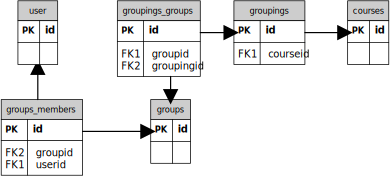
\includegraphics[width=\textwidth]{images/moodlegroups}
	\label{fig:moodlegroupsandgroupings}
	\morscaption{The database scheme for groups and groupings. Non primary key and non foreign keys data fields is omitted for brevity}  
\end{figure}

This structure supports that users can be in groups and that more groups can be grouped together in one grouping. 
One group can be a part of several groupings and an user can be a member of several groups. 
The foreign key from groups to course and the foreign key from grouping to course indicates a tight connection between groups and courses. 

\subsection{Plugin}

As mentioned in \secref{sub:lms} the M in Moodle stands for modular. 
The Moodle development staff made 34~\cite{plugins} types of plugins.
We will explain four of the most common: 



%http://docs.moodle.org/dev/Plugins


\paragraph{Blocks}
\label{subsec:blocks}
%http://docs.moodle.org/dev/Blocks
Moodle use the term block to refer to a box that can contain a wide spectrum of information and functionality.
A block can as default be placed in the left or right side of a page. 
The navigation block is a very common block which as default is displayed on all pages. 
It contain links such as: My Profile and Courses. 
Blocks are not limited to navigational purposes but can also display data from the database.

Each block have settings regulating on which pages it can displayed. Block can be places in number of different regions if the theme allows it. 

``Small information-displays or tools that can be moved around pages''
%Hvornår er det godt at lave en block
%http://phpdocs.moodle.org/HEAD/core/lib/moodle_page.html
%http://phpdocs.moodle.org/HEAD/moodlecore/moodle_page.html



\paragraph{Activity modules}
%http://docs.moodle.org/dev/Activity_modules
%http://docs.moodle.org/22/en/Activity_modules
%http://docs.moodle.org/22/en/Activity_modules_administration
``An activity is a general name for a group of features in a Moodle course.''~\cite{activity} 
Activity modules are the main way to create new features in a course. 
It is common that a course page contains a activity block~\cite{}
show table 
hvornår skal man lave et am

``Activity modules are the most important type of plugins. They provide activities in courses. For example: Forum, Quiz and Assignment.''
\paragraph{Admin Tools}
%http://docs.moodle.org/dev/Admin_tools

hvad er det
hvem har rettigehder

hvornår skal man lave et admin tool

``Provides utility scripts useful for admins to examine and modify a Moodle site''
\paragraph{Local Plugins}
%http://docs.moodle.org/dev/Local_plugins
hvad er det
properties

``Generic plugins for local customisations''



\subsection{Framework}
Moodle includes various APIs~\cite{moodlecoreapis}, which aids the developer in the process of creating application. Some of the APIs are:

\begin{itemize}
	\item Data Manipulation (DML) API~\cite{moodledml}. Used for all data access and is described further in \secref{sec:moodleoplatformdbml}
	\item Form API~\cite{moodleformapi} for rendering HTML form objects and handle the validation of the data send through the form. 
	\item Output API~\cite{moodleoutputapi} for general HTML rendering.
	\item Page API~\cite{moodlepageapi} for setup of a standalone page including methods for adding javascript and configuring display options. 
	\item Access API~\cite{moodleaccessapi} for controlling access levels of users throughout the Moodle. 
	\item Unit test API~\cite{moodleunittestapi} for testing components in Moodle. 
\end{itemize}
Moodle APIs are used in different ways. The DML, page, and output APIs are used through global variables, whilst others are used through class extensions. In~\coderef{moodleapiusage} the page and form APIs usage is shown.
\begin{lstlisting}[style=phpCode, caption=\myCaption{Example of the Page and form APIs in Moodle}, label=moodleapiusage]
$PAGE->set_context($somecontext);

class some_form extends moodleform {
	...
}
\end{lstlisting}


\subsubsection{Database Layer}
\label{sec:moodleoplatformdbml}
To access and manipulate data in Moodle the DML API is used.  The API is accessed through a global variable named \$DB. It has several method for update, insert, delete, and select. 
The basic method for select, insert, and update, namely get\_record, update\_record, and insert\_record, take or retrieves an object of type StdClass\todo{Hvor  skal StdClass forklares?}. This gives a unified procedure for manipulation data. A simple update procedure is seen in \coderef{moodlecodeupdate}.
\begin{lstlisting}[style=phpCode, caption=\myCaption{Example of how to change the name of an user}, label=moodlecodeupdate]
function change_name($id, $new_name){
	global $DB;
	$user = $DB->get_record('user', array('id'=>$id));
	$user->name = $new_name;
	$DB->update_record('user', $user);
}
\end{lstlisting}
For simple operations no SQL is needed, but for more complex queries such as queries using joins SQL most be written directly. 



\subsubsection{Context System}
\label{sub:contextsystem}
The context system in Moodle is used to set the context of a given page to determine the users capabilities and which blocks to present~\cite{moodlerolesandmodules}.
 
When a user is logged in to a Moodle system he can have various roles in various contexts. 
One person might be a student in one course and a teacher in others. 
Moodle use a hierarchical context system to manage users roles and their capabilities. 
The context systems hierarchical layout can be seen in \figref{fig:moodle-contexts}~\cite{moodlefilemoodlecontext}.
 
 \begin{figure}
	 \centering
		 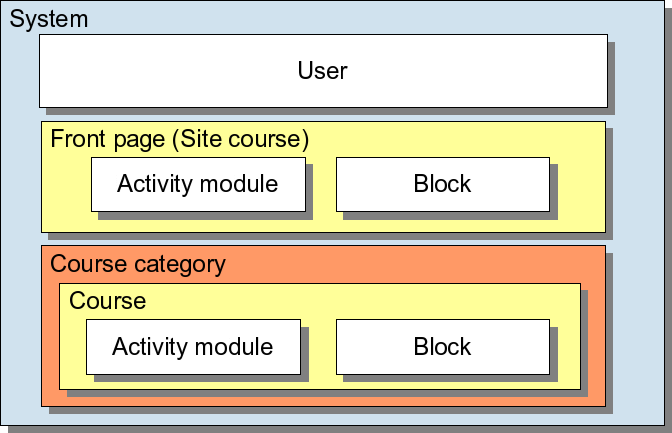
\includegraphics[width=\textwidth]{images/moodle-contexts.png}
	 \label{fig:moodle-contexts}
	\morscaption{The hierarchical context structure in moodle}
 \end{figure}

The highest level of context is the system context which all inherit from. 

Every page in Moodle which is loaded directly through HTTP(S) must set the page context. 
An example of how to set the context can be seen in code snippet \ref{courseviewcontextsnippet} from \moodlefile{/course/view.php}, which loads the default page of a Moodle course.

\begin{lstlisting}[style=phpCode, caption=\myCaption{A snippet from \moodlefile{/course/view.php}}, label=courseviewcontextsnippet]
...
if (!$context = get_context_instance(CONTEXT_COURSE, $course->id)) {
  print_error('nocontext');
}
...
if ($switchrole > 0 && confirm_sesskey() &&
  has_capability('moodle/role:switchroles', $context)) {
...	
\end{lstlisting}
The function \fu{get\_context\_instance} requires a constant and in this case a course id. 
the constant used for the function is a constant telling which context level that needs to be loaded. This is a numeric value. 
In this example an error is outputted if the context fails to load. 
To determine whether or not an user has the capability to do certain actions the function \fu{has\_capability} is used~\cite{moodlerolesandmodules}. It requires a string specifying which capability and the context for the current page. 
It i required to set the context for each page. 
In some pages Moodle sets the context itself~\cite{moodlepageapi}. 

Beside being responsible for capabilities contexts are used to determine the presented blocks on a page. If an user with the capability to edit a course page adds a block and the instance is set to the system context the block will be showed on all course pages. If the context is set to the course context the block will only be presented on that courses page. 

	
	
	
\chapter{Development Practices} %remember to say how we work with costumers
\label{sec:developmentpractice}
\myTop{This chapter gives a description of how we are using the development method Scrum of Scrum.
Where \secref{sec:devMethod} is regarding the development method of the entire group, this chapter regards how we are implementing the development method in our \subgroup{}.
There is some repetition from \secref{sec:devMethod}, to recall the decisions made previously.}

%As described in section \ref{subsec:choosingmethod} we have chosen to use Scrum of Scrums with some changes.


\section{Adapting the Development Method}
%\section{Choosing a Development Method}
%because many people -> agile. our version of scrum

%We need a development method that takes the large number of people we are into account.
%Furthermore, the development method also needs to take into account that we are working on a platform (namely Moodle), which most of us are unfamiliar with.

%We choose to use the development method Scrum (see section \ref{par:scrum}) with a few changes.
%he reason why we cannot use Scrum in its original form is that we do not have all the required personnel. 

Scrum requires an on-site costumer and a product owner.
We have neither, so we have to make some modifications to the development method.
Instead we have acquired some customers from which we get requirements and feedback for the system we are developing.
As the \groupname{} we are responsible for creating the administrative part of the system as well as creating the virtual meeting place, as described in \secref{sec:admgroupdecom}.
Therefore we are in contact with administrative personnel at Aalborg University, which serve as costumers.

The costumers for the functionality of the group page are the three other groups in this multi-project.
How we work together with our costumers will be described later in this chapter.

\section{Utilizing the Development Method} %TDD MANGLER STADIG ET STED I DENNE section SKAL DEN VÆRE HER?
%utilizing agile methods -> we don't know shit so its good
Since we are not familiar with Moodle, from the beginning of the project we do not have a full understanding of how the entirety of the system should be structured and created.
We solve this problem by dividing the development process into a number of sprints.
Ideally after each sprint we should have a fully functional system, which is in such a state that it can be shipped.
This is not entirely the case, since we need a lot of information before we can start programming.

%sprints
To handle this our first sprint will consist of information gathering; we study the Moodle platform as well as interview our costumers in order to get requirements.
%product backlog
These requirements are used to create feature descriptions, which are used to fill the product backlog.
%sprint backlog
At the beginning of each succeeding sprints in our group we choose items from the product backlog and move them to the sprint backlog, which is a list of features we expect to implement in the particular sprint.

%planning poker
In order to choose which items to move to the sprint backlog we assign each item currently in the product backlog a number of story points.
We do this by playing planning poker, which is a card game where we all give our estimates of the items on the backlog simultaneously, and then discuss the estimates if there is a significant difference between us.

%burndown chart
As we progress in the sprint the number of remaining number story points starts to dwindle. 
We keep track of this by a burn-down chart, which is a physical chart with a line that shows the expected progress.
The total number of remaining story points are plotted into the graph each day, so we can see if we are progressing at a satisfactory rate.

%daily scrum
In our group we start each day with a scrum meeting.
In this short meeting we all stand up and each tell three things: What we did since last scrum meeting, what we are going to do today, and which -- if any -- impediments we have.
This gives the entire group and idea of what is being worked on, and by doing this everybody always have a task they have chosen themselves.

\section{The Development Method Across Groups} %change this title if you are so fucking clever that you think you can do better
Since we are dependent on each other across the groups in the multi-project, we need to organize what each group is doing.
We do this in two ways: in between sprints and during sprints.

%sprint planning meetings
At the beginning of each sprint all the groups present their plan for what they are going to produce in the coming sprint.
If other groups have any dependencies, they communicate these and the groups collaboratively decide the overall tasks each group should accomplish in the given sprint.

%demo meetings
At the end of each sprint the groups meet and present what they have created during the sprint.
Depending on the state of the system costumers can be invited to these meetings.
Otherwise costumers can be invited to try or be showcased specific aspects of the system by individual groups.

%weekly casual scrum og scrum meetings
During sprints the groups still work together to some extent.
Since we all work close to each other we can always go to another group room to ask for help or request that some specific work should be done.
Additionally we hold Scrum of Scrums meetings at an approximately weekly rate.
In these meetings the Scrum masters of all the groups meet and discuss the direction of the project and share information regarding how the system should be integrated with the different components that the groups are developing.
	
	\chapter{Analysis}
\label{chap:analysis}
\myTop{In this chapter we present our analysis of the platform on which our final system depends and the concept of project groups.
In \secref{sec:moodleplatform} concepts of Moodle are presented and analyzed.
We introduce the concept of project groups in \secref{sec:projectgroups}, where different aspects of a project are considered.
Decisions are not made in this chapter, rather a foundation is build to allow design and implementation decisions in later chapters.}


\section{Projectgroups}
\subsection{Manage Project Group}
\subsubsection{Current Systems}
\subsubsection{Possible Future Systems}





\begin{comment}
\todo{Undersøgelse af: "`Hvem skal oprette projektgrupperne"' }
\todo{Kom frem til at vi skal interview administrativt personale for at finde ud af hvordan grupper bliver brugt i praksis}
\subsection{Interviews}
\todo{Fortæl om følgende interviews
-Thomas Rybjerg
-Lene Even
-Jette og Pia
-Morten Andersen
-Mikael Møller} 
\end{comment}


	
	\chapter{Design}
\label{chap:design}
\todo{header}

\section{Architecture}
\label{sec:architecture}
\system{} is an extension of \moodle{} and can be seen as a package of plugins. 
The architecture does not specify how each plugin should be created, but specifies a general structure of the components of the system. 
The complete architecture can be seen in \figref{fig:architecture}.
\begin{figure}[h!t]
	\centering
		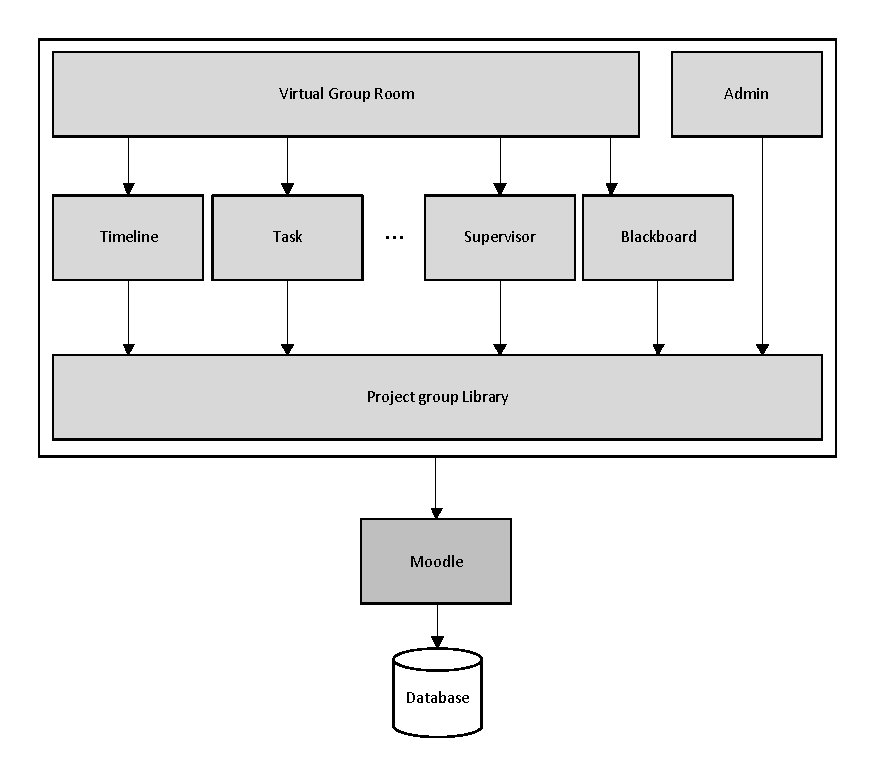
\includegraphics[width=\textwidth]{images/architecture.pdf}
	\morscaption{The overall architecture of MyMoodle}
	\label{fig:architecture}
\end{figure}

The architecture consists of a total of five layers. 
The three uppermost constitute \system{}, they have a common dependency, namely the Moodle platform. 
Layers four and five are Moodle and the Database system respectively.
%Our extension  as a plugin of Moodle and use functions supplied by Moodle to function.

We explain the three uppermost layers as:
\begin{enumerate}
	\item The uppermost layer is the virtual group room and the administration tool.
	%The virtual group room is used for presenting the virtual meeting place for a project group.
	The virtual group room is described in \secref{sec:virtualMeetingPlace}.
	The administrative tool is used by administrative personnel for managing project groups.
	It is described in \secref{sec:groupManagement}.
	This layer is called ``View Layer''.
	\item Directly below the uppermost layer is the middle layer, which consists of the four components: Timeline, Task, Supervisor, and Blackboard.
	These four components are created by our peer-groups and are not explained further.
	We call this layer ``Content Layer'', since the components in this layer generate content for the virtual group room component.
	This layer has three dots in the center in order to show that there exist more components and more can be added here. 
	%An example is the \detdeandrelaver{} that presents the members of the project group. 
	\item Below the Content Layer is the project group library, which contains common functionality.
	This layer handles all communication between the components in the Content Layer.  
	We call this layer the ``Library Layer''.
\end{enumerate}


There are two primary factors we need to consider when planning our architecture. 
Firstly, we are four sub-groups working together. 
This creates the need for a structured way of communicating between the different component and it lets every \subgroup{} know how their component is connected to the rest of the project. 
Secondly, the project should be passed on, which requires an architecture that grants great comprehensibility and extensibility of the project.
%alex -> <@:-D-|-<

It is not possible to make a strict layered architecture due to the Moodle dependency, and the administrative tool, which does not have to use the Content Layer, but depends directly on the project group library and \moodle{}.
We do, however, prohibit ourselves from accessing the database directly, by using the Moodle Database Layer (note that it is not a layer in our architecture) described in \secref{sec:moodleoplatformdbml}.
In \figref{fig:architecture} the dependency from the box encircling \system{} indicates that every component in \system{} depends on the \moodle{} component.
The \moodle{} component consists of the Database Layer as well as the Context System, Capabilities, etc.

%These considerations leads us to design the illustrated architecture in \figref{fig:architecture}.
Note that the relative size of the components do not imply anything, e.g.\ the Moodle component is code wise much larger, than all of the components in \system{} combined, but is illustrated with a rectangle the same size as any of the Content Layer components.














\section{Project Group}
\label{sec:projectgroup}
In this section the different aspects of the concept of the project groups will be described.
First we want to introduce the concept of a virtual meeting places for project groups.
How to navigate through the project groups is described afterwards.
Finally the design decisions regarding management of project groups is described.
\todo{Tjek igennem når analysen om dette emne er lavet }

\subsection{The Virtual Meeting Place}
The members of a project group should have a place where they can meet and engage in project related activities.
Recall from \secref{sec:subSysDef} that our responsibility is to construct a place where this can happen, not construct the actual activities -- that is the responsibility of our peer-groups.
We have to decide the scope of the virtual meeting place.
For example who should be able to see the work in progress of a project and who should be able to modify it.
One idea is to have every project share everything with other projects.
This corresponds to having every project group working in the same room in the real world.
Another idea is to give a virtual group room to every project group and ensuring that only the members of the project group and the supervisors can contribute to the work on the project.
The corresponding situation in the real world is that every project group has their own group room where only they (and there supervisors) can do work on the project.
The first idea is easier than the second to implement since no permissions need to be considered.
However, the second idea is closer to the way that Aalborg PBL is implemented -- with a team working together on the project as described in \secref{sub:aaupbl}.

We choose the second idea.
It is simply too infeasible to have every project group share everything.
A project group member could be forced to look through many functionalities to find the one relevant to the given project group.
Furthermore, by allowing each project group to have there own virtual group room, the members can customize the place as they see fit by removing irrelevant functionalities and possibly adding new relevant functionalities.
For the rest of the report we refer to the virtual group room simply as the ``project group room''.

The project group room should have some of the same functionality as a physical group room.
We as the \groupname{} implement the page, and the other three peer-groups implement the blocks (see \secref{subsec:blocks}) that serve as different functionality.
A good aspect of using blocks is that it is easy to manage which blocks should be shown and where they should be shown on the page.
The project group room is a place where students can exchange information among themselves and with their supervisor.

\subsection{Navigation}
\label{sub:designprojectgroupnavigation}
There is currently a problem in Moodle when it comes to navigation. 
When a user is enrolled in a large number of courses their entire front page is filled with links to those courses.
There is no built-in functionality to move or sort the links.
ELSA mentioned this problem during the meeting that we conducted with them described in \secref{sub:elsaInterview}.
%ref Lene
\todo{insert refs to interview with Lene. Hvorfor til Lene når det er ELSA der omtales?}

We want to avoid this problem when we design the navigation for project groups.
Moodle has a navigation block with a list of important links.
We want to add an item to this list that, when expanded, shows the project groups the user is a member of.
Since a supervisor or an administrator might be a member of a many project groups, we want to limit the size of the list of project groups.
We do this by showing at max a preset value, and if the user is a member of more groups we show a link to a page that has a list of all the users's group.

\subsection{Managing Project Groups}
\label{sec:s}
Administrators need to be able to add, remove, and edit project groups.
Per default Moodle has a block called Settings. 
If a user is an administrator there is a list in this block called site administration. 
This list contains a lot of tools administrators use, and it is only natural to add project group administration to this list. 

We want a page where administrators can add a new project group that also adheres to Moodle standards.
It should be possible to name a group, add the desired members, and choose who the supervisor(s) of the group is/are.

Additionally there needs to be a list of all project groups.
This list can potentiality grow very large, so there needs a way of finding a specific group or a specific set of groups. \todo{lene interview ref}
From this list it should be possible to add, edit, and delete groups. 

The project group administration should be implemented in such a way that it does not decrease the efficiency for the administrative personal compared to the old system. 
This measure can only be used in placed where an existing project group administration system is used.
\section{Database}
\label{sec:dbdesign}
In this section we will present the design of our database.
Our design will support the concepts that we have introduced, namely project groups and project group members.

Recall that we are designing to comply with a relational database, more specifically an SQL database as described in \secref{sub:constraints}.

\subsection{Project Group table}
\label{sub:dbProjectGroup}
A project group is an entity that consists of different elements.
How these elements are represented in the database is described here.
One core element is the project group members, this is described in \secref{sub:dbProjectGroupMembers}.
The other elements will be represented as fields in the \rel{projectgroup} relation.
%The reason for this is that a project group is an entity that has some attributes which we want to save persistent.

A project group must be identifiable by both human and computers.
To make a project group identifiable by humans we give it a short name that must be unique among other project groups.
The field that holds the short name in the project group relation is called \field{shortname}.
Initially it may seem that the short name could be used as a general identifier (both for humans and computers) since a short name is unique.
However, this name might be changed during the lifespan of a project group.
We much rather prefer an identifier that is constant for a project group to a avoid race conditions. 
%and violations of referential integrity
An example of a race condition in this system could be a user trying to access a project group with an identifier (the short name in this case) while another user is changing the short name of the group.
Should the short name be changed before the first user is trying to access the project group.
The request will fail because the identifier that he is holding is deprecated.

We choose to have a numeric auto-incrementing \field{id} field to identify the project groups.
This cannot be set or changed by the users of the system.
%Ultimately a databse administrator could change it directly in the database, but we cannot guard gainst this assuming the database administrator has super user privelges.
It is a Moodle guideline to have an auto-incrementing field as primary key~\cite{moodledb}.
We clearly obey this guideline by making \field{id} the primary key of \rel{projectgroup}.

One could argue that the numeric id field could be used as human identifier as well.
However, we deem it much easier for a humans to remember and associate an alphanumeric name with a particular project group than an arbitrary number.
In summary a project group has two identifiers; the numeric \field{id} and the alphanumeric \field{shortname}.
The former being the primary key of the relation.

To give a better description of a project group, we have an optional field called \field{longname}.
This field does not need to be unique, but only serves as a description for a project group.

To allow project groups to be ordered or filtered based on which semester (or another time-based constraint) they belong to we choose to have a timestamp field called \field{created}.
The value of this field is the Unix-timestamp at the time of the creation of the project group.

The four fields of \rel{projectgroup} are as follows.
\begin{itemize}
	\item \field{id} to identify the group.
	\item \field{shortname} to easily identify the group for humans.
	\item \field{longname} of the group, for a more descriptive name.
	\item \field{created} timestamp for a given project group.
\end{itemize}

An instance of \rel{projectgroup} with a single tuple (representing our own group) is shown \figref{fig:projectgrouprel}.
Notice in the figure that \field{shortname} might seem somewhat cryptic.
It translates to: ``Software Engineering, 6\ths{} semester, group number 8, spring (for\aa{}r), 2012''.
This illustrates the need for \field{longname}, since supervisors might find difficulty distinguishing several groups of the same semester simply by their group number.
\field{longname} gives a more descriptive name that should clearly give an idea of which it project group is.

\begin{figure}[htb]
	\centering
		\begin{tabular}{|l|l|p{0.5\textwidth}|l|}
			\hline
			\field{id} & \field{shortname} & \field{longname} & \field{created} \\
			\hline
			1 & SW608F12 & \groupname{} working on \system{} & 1337723013 \\
			\hline
		\end{tabular}
	\morscaption{Example of an instance of \rel{projectgroup}}
	\label{fig:projectgrouprel}
\end{figure}


\subsection{Project Group Members table}
\label{sub:dbProjectGroupMembers}
As opposed to a project group a project group member is not an entity in its own right.
A project group member is a user that is a member of a project group.
\moodle{} saves users in a relation named \rel{user}.
This relation contains information about the users of the system -- a unique identifier in particular -- and is part of the \moodle{} core database schema~\cite{moodledbschema}.
We want project group members to be represented in the database as a link between \rel{projectgroup} and \rel{user}.
We want this link to be many-to-many, since a project group can contain many members and a user can be a member of many project groups.

We can save the link in either \rel{user} or \rel{projectgroup}, or create a new relation to save them in.
We state in our system definition (seen in \secref{sec:systemDef}) that current functionality of \moodle{} should not be altered.
The first alternative is therefore out of the question since we cannot guarantee that the other parts of \moodle{} will continue to work as before if we alter in the core database relations.

Should we choose the second alternative we would make $n$ fields in \rel{projectgroup}, each containing a member of the project group or a value indicating no members, e.g. as null.
This would set a maximum of $n$ members on every project group.
If there is a maximum number of members that will ever be in a project group and this number is acceptably low this alternative might be viable.
%We do not, however, know any such number.
The number of users in the system could be a candidate for a maximum value.
This number may, however, change as more users are added to the system.
Furthermore, this number is likely to be larger than the actual maximum number of members in any group, assuming that no or few projects are conducted by every user of a \moodle{} system.
Another option is to choose a value that we believe is high enough for most purposes.
This would result in a many-to-$n$ link between project groups and users, in that a project group can have $n$ members and a user can be a member of any number of project groups.
If this $n$ value is chosen to high, space will be wasted, e.g. if $n$ is set to $20$ and no project group ever has more than 10 members, at least 10 fields in each \rel{projectrgoup} tuple will be wasted.
If $n$ is too low the system will be unacceptable because some desired project groups cannot be created.

The final alternative requires a new relation which stores a combination of users and project groups.
This allows for a true many-to-many link between users and project groups.
By choosing this alternative we have great extensibility, e.g. we are able to save the role of project group member in this relation as well.
A weakness to choosing this alternative is greater complexity by an increase in the number of relations.
The strengths of this alternative outweighs its weaknesses and it is better than the previous alternative by allowing a true many-to-many link without wasting space or making the system unacceptable.
Hence we choose this alternative as the way to save project group members in the database.
The relation that is used to link \rel{user} and \rel{projectgroup} is called \rel{projectgroup\_members}.

%%%%%%%%%%%%%%%%%%%%%%%%%%%%%%
% M�ske skal vi inds�tte en  %
% sub-subsection her         %
%%%%%%%%%%%%%%%%%%%%%%%%%%%%%%

For \rel{projectgroup\_members} to link \rel{user} and \rel{projectgroup} it will have a foreign key to both of these relations' primary keys.
The fields that hold these foreign keys are called \field{user} and \field{projectgroup} respectively.
The combination of \field{user} and \field{projectgroup} is a candidate key for \rel{projectgroup\_members}.
However, as with \rel{projectgroup} we choose to have a numeric auto-incrementing single field called \field{id} to comply with \moodle{} guidelines~\cite{moodledb}.
We still make the combination of \field{user} and \field{projectgroup} unique, to ensure that no person is a member of the same group more than once.

Whenever a user is a member of a project group we want to have a role associated to that member.
We can choose to give every user a role and whenever that user is a member of a project group he can act and have privileges as fit for the role.
Another way to do it is to save the role along with the link between users and project groups.
We prefer the latter for two reasons.
Firstly a user may have different roles in different project groups, e.g. a Ph.D. student has a student role in his Ph.D. project, but may also be supervising projects being conducted by younger students.
Secondly we would have to make a new relation to contain only this information and thus increase complexity if the former alternative is to be chosen.
We will not alter the core relations such as \rel{user}, as described in \secref{sub:dbProjectGroup}.

To allow for extensibility we save the creation and update time of each tuple in \rel{projectgroup\_members} in \field{created} and \field{updated} respectively.
It may be useful to have these timestamps for administrative personnel, e.g. to see whether or not a user has joined a project group later than the other members.

The final set of fields in \rel{projectgroup\_members} are:
\begin{itemize}
	\item \field{id} which is Moodle convention. \cite{moodledb}.
	\item \field{projectgroup} references to the related project group.
	\item \field{user} references to the related user.
	\item \field{role} denoting the type of membership the user has to the group.
	\item \field{created} is the timestamp for its creation.
	\item \field{updated} is the timestamp for the last update to the membership. 
\end{itemize}

\figref{fig:projectgroupmembersrel} shows an instance of \rel{projectgroup\_members} containing four students (indicated by role ``0'') and a supervisor (indicated by role ``1'').
Notice that all tuples have the same \field{projectgroup} value.
This indicates that every tuple links user to the same project group, namely the one shown in \figref{fig:projectgrouprel}.

\begin{figure}[htb]
	\centering
		\begin{tabular}{|l|l|l|l|l|l|}
			\hline
			\field{id} & \field{projectgroup} & \field{user} & \field{role} & \field{created} & \field{updated} \\
			\hline
			1 & 1 & 1 & 0 & 1337723013 & 1337723013 \\
			\hline
			2 & 1 & 2 & 0 & 1337723013 & 1337723013 \\
			\hline
			3 & 1 & 3 & 0 & 1337723013 & 1337723013 \\
			\hline
			4 & 1 & 4 & 0 & 1337723013 & 1337723013 \\
			\hline
			5 & 1 & 17 & 1 & 1337723184 & 1337723184 \\
			\hline
		\end{tabular}
	\morscaption{Example of an instance of \rel{projectgroup\_members}}
	\label{fig:projectgroupmembersrel}
\end{figure}


The database scheme can be seen in~\figref{fig:projectgroupsdb}. 
The user entity is a built-in part of Moodle and is not modeled by us. 
\begin{figure}
	\centering
		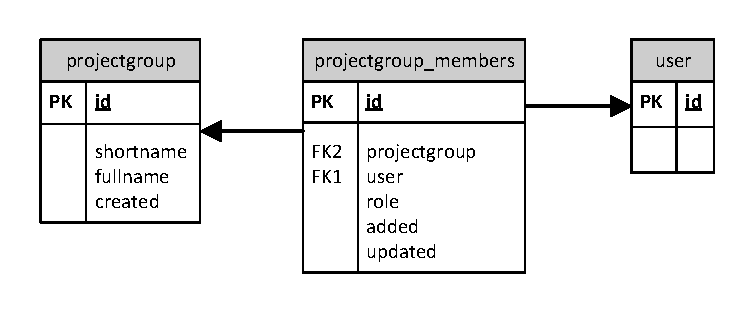
\includegraphics[width=\textwidth]{images/projectgroupsdb.pdf}
	\morscaption{The database scheme of project groups and memberships.
	Most of the data fields of the user table are omitted for brevity.
	The user table consist of more than 50 fields}
	\label{fig:projectgroupsdb}
\end{figure}

%To test the scheme for redundancy we check to see that the scheme conforms to boyce-codd normal form (BCNF). To check this we 




\begin{comment}
\todo{central controlled groups vs student create groups}
\section{Platform}
	%About moodle
\section{Architecture}
	%Overall architecture of the entire MyMoodle system
\section{Administrative Subsystem}
	%In the system we want projects to be independent...
\section{Database}
	%ER-diagrams 
\end{comment}
	
	\chapter{Implementation}
\newcommand{\viewroom}{}
\myTop{In this chapter we describe how we implement the concepts described in \secref{chap:design}.
%This chapter is divided into three sections where the two main parts of our system are described, namely \nameref{sec:projGroupRoomImpl} and \nameref{sec:manProjGrpImpl}.

The implementation details presented here are paramount for \chapref{chap:test} and \chapref{chap:evalProduct}.}
From section \secref{sec:architecture} we know there is three part which must be implemented by us. 
The administration tool to manage project group, the project group, and the project group \viewroom. 
The administration tool is implemented as an admin tool, which as described in \section{platform} is a special moodle plugin type. 
Project groups can be implemented as courses (see \secref{sub:courses}) by creating a new view for the course page. 
Hereby solving the problem of both implementing project groups and the aforementioned project group \viewroom.
This will make it possible to use activity modules, described in \ref{par:activitymodules}, in the project group. 
Another approach is to make a local plugin, which gives us basic functionality, such as database installation. 
With a local plugin we cannot use activity modules since they are too strongly connected to courses. 
Instead we can use blocks for the functionality. 
The later approach is chosen. 
The local plugin includes both the project group library and the project group  \viewroom. 
The view is implemented in the file \moodlefile{/local/projectgroup/view.php} and  the library is in the file \moodlefile{/local/projectgroup/lib.php}. 
The library includes several other files. 
One for each sub group and several helper files. 

\section{Project group library}
The project group library is build up by several files and consist of several functions and classes.
It is shared between all subgroups. 
This section only explains the functionality implemented by our subgroup. 
%% Lines of codes
%% How many functions

In the following sections is how we put our project group into a moodle context and how we ensure permissions.

\subsection{Overwrite Context}
In \secref{sub:contextsystem}  the context system of Moodle is described.
In this section the creation of a custom context is described. 

To be able to define capabilities for the project groups and have different blocks for different project group we need our own context.
We will create our own context level and class.
We call the context \cl{context\_projectgroup}. 

Moodle does not support extension of contexts through one of the more than 30 different plugin types available \cite{plugin}. 
There two parts of the problem, the first is to create a new context and the second is to load it properly. 
We create a new context by making a new class which is very similar to \cl{context\_course} class and by defining the context level of project groups as a constant. 
The class header and the constant definition can be seen in \coderef{codeprojectgroupcontext}. 
The constant is set to 55 and is chosen because that context level is unused and it is close to the course context level. 
We regard the project group contexts to be at the same level as course contexts. 
However, project groups does not have categories like courses does.

\begin{lstlisting}[style=phpCode, caption=\myCaption{The context\_projectgroup class header and constant definition}, label=codeprojectgroupcontext]
define ('CONTEXT_PROJECTGROUP',55);
class context_projectgroup extends context {
...
\end{lstlisting}

When a context is loaded in a Moodle page it is instantiated by \fu{get\_context\_instance}, which takes a context level and an instance id. 
The instance id can be a course id or similar depending on the context level -- in our case it is a project group id. 
This function calls a static method in the \cl{context\_helper} class which uses a private array to translate the context level into a class name.
The overall system definition in \chapref{chap:systemDef} retain us from changing the core code of Moodle. 
If this constraint were not enforced the array could simply be extended directly in the code.  
Since the array used is private we can not extend the context system by overriding the \cl{context\_helper} class. 
The newly created context is only used in pages created in this project and we can therefore create our own version of \fu{get\_context\_instance}. 
The new function can be seen in \coderef{codeprojectgroupcontextinstance}.
\begin{lstlisting}[style=phpCode, caption=\myCaption{The function to get projectgroup context}, label=codeprojectgroupcontextinstance]
function get_projectgroup_context_instance( $instance = 0, $strictness = IGNORE_MISSING) 
{ 
    return context_projectgroup::instance($instance, $strictness);
}
\end{lstlisting}
The \vari{instance} variable denotes a project group id.
The \vari{strictness} variable 

With the new context and the function to instantiate it we can now make per project group permissions and add blocks to specific project group pages. 
\subsection{Ensuring Permissions}
\label{sec:projectgrouproommanagerights}
Permissions can generally be divided in two types; read and write. 
Read permissions gives you the ability to view the content of the virtual group room while write lets you change the content. 
If a user has write permission he must also have read permissions, otherwise he cannot see the page he attempts to edit. 
To ensure the user attempting to enter a virtual group room has permission to enter the function \fu{has\_projectgroup\_read\_permission} is used. 
%It checks if the user is a member of the group. 
It checks if the user is an administrator or is a member of the project group. 
The administrator check is necessary since an administrator should be able to see any project group even if he is not a member of the project group. 

The function \fu{has\_projectgroup\_write\_permission} checks that the user has write permissions and uses the read permission function to check that the user has read permission.
If he does not have read permission he should not be able to edit the virtual group room. 
In the current implementation the write permissions function does not make extra checks to permissions since the permission levels for read and write are equivalent.

Because the functions are separate it is possible to change them individually later.
%Making both function gives the ability to later change this.
An example is that an end users requires that supervisors should only have read permissions. Then the change will only be in one place. 
Both functions can be found in the project group library.


\FloatBarrier

In the implementation of the project group we are faced with several choices. 
Project groups can be implemented as courses by creating a new view for the course page.  
This will make it possible to use activity modules, described in \ref{par:activitymodules}, in the project group. 
Another approach is to make a local plugin, which gives us basic functionality, such as database installation. 
With a local plugin we cannot use activity modules since they are too related to courses. 
Instead we can use blocks for the functionality. 
The later approach is chosen. 

\section{Project Group Room}
In this section the actual implementation of the project group room, its custom blocks, how the context system is used to implement our own context to allow better administration of blocks and capabilities, and the navigation to the users project groups is described.
The section presents how the project groups work from the perspective of the user. 


\subsection{The page}
The project group page is the virtual meeting place described in \secref{sec:projectgroup}.
We decided to implement the room merely as a container for blocks. 
Alternatively the functionality could be an integrated part of the page, but using blocks gives more flexibility to the users allowing them manage the layout of their own project group room. 
A screenshot of a project group room can be seen in \figref{fig:projectgroupnoedit}. 
In this project group room the blocks are layouted as they are per default. 
\begin{figure}[h]
	\centering
		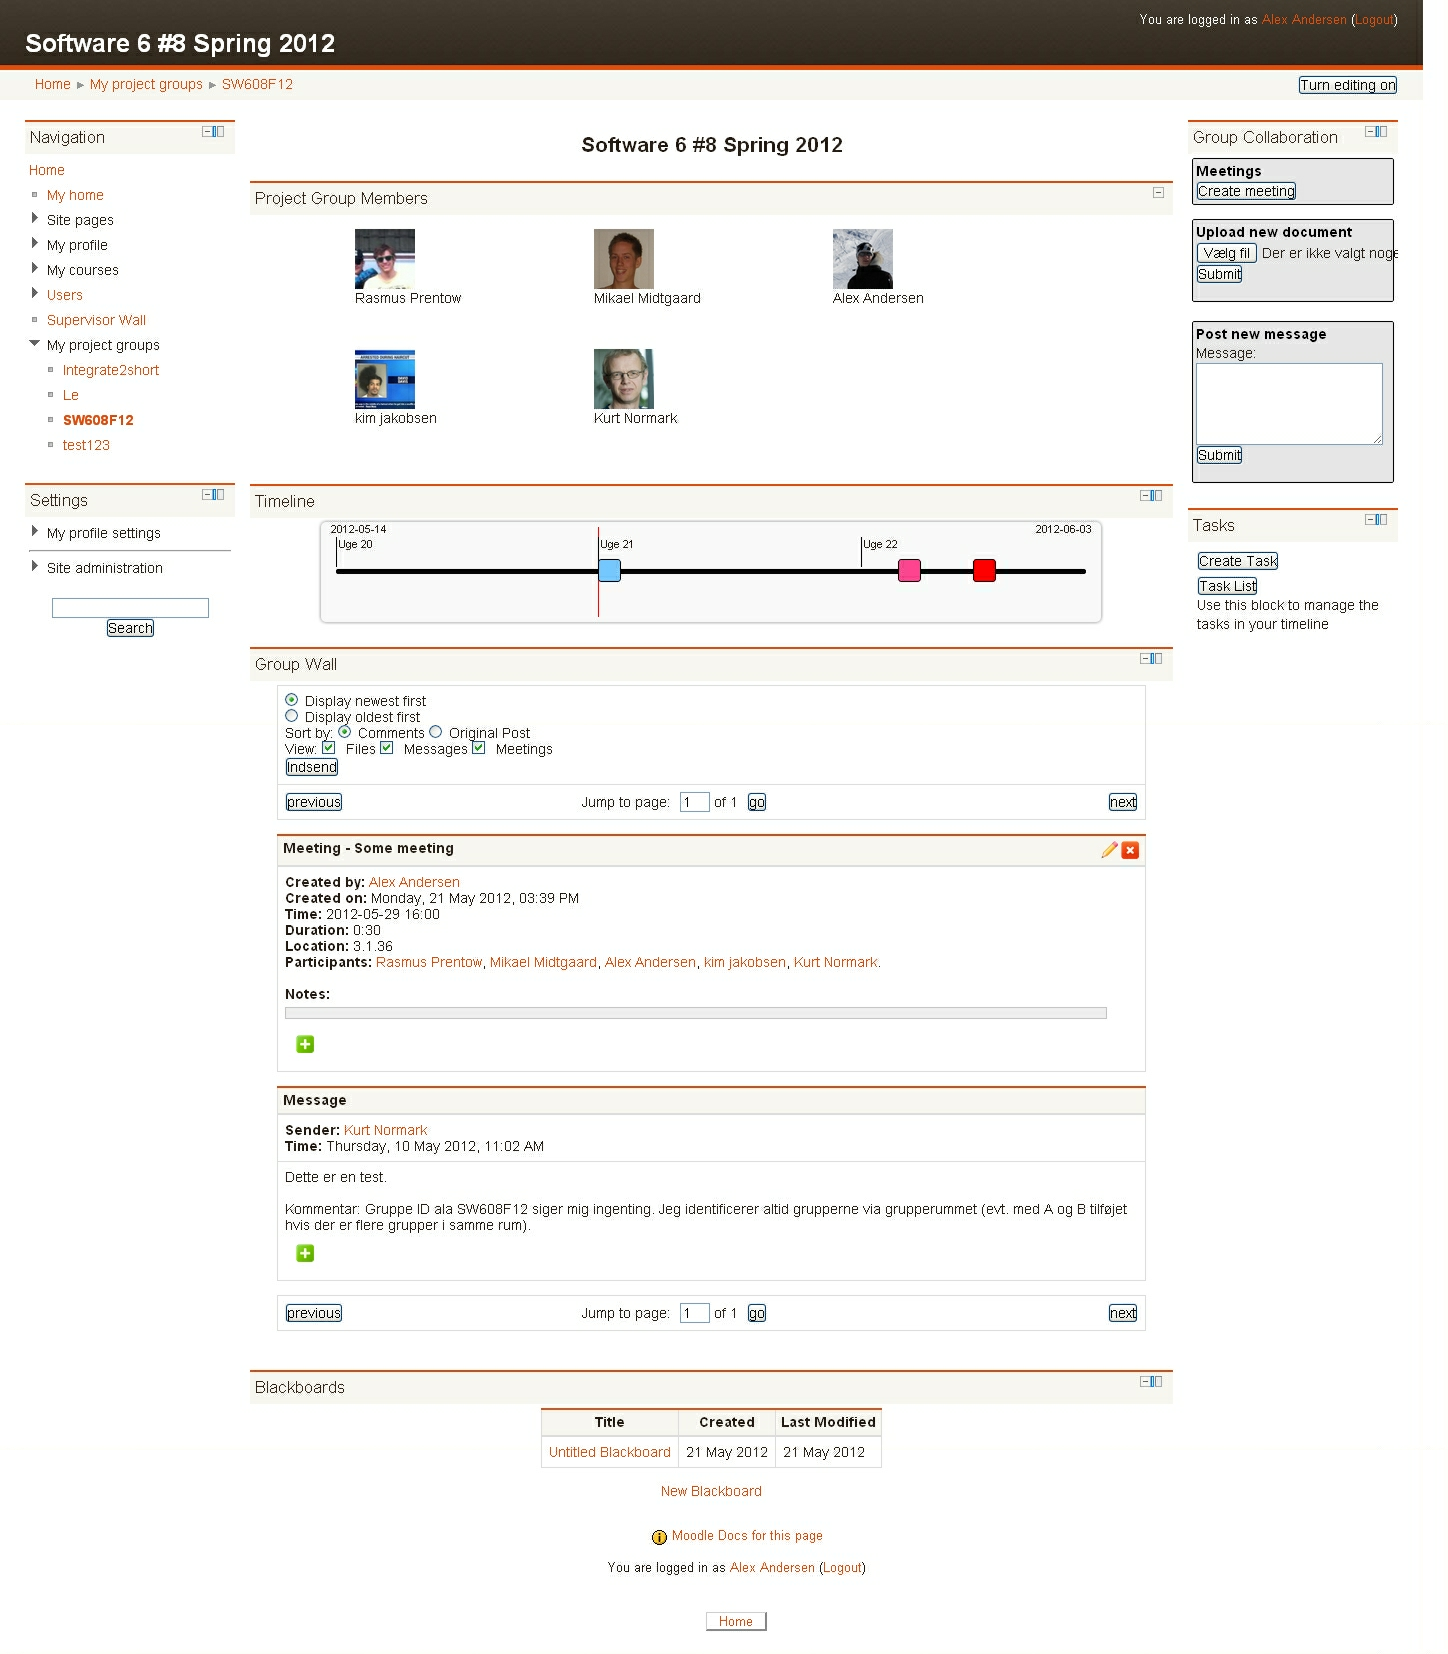
\includegraphics[width=\textwidth]{images/projectgroupnoedit.png}
	\morscaption{The project group room}
	\label{fig:projectgroupnoedit}
\end{figure}

The project group room consist of three columns. 
The left column is the standard navigation menu in Moodle. 
The Center and right columns both contain blocks.
The various blocks presented on the project groups page is described in \secref{sec:implprojectgroupblocks}. 
If an user wants to edit the block layout for the project group room he can press the ``Turn editing on'' button. 
This will add edit and move buttons to each block. 
A new block is added in editing mode to allow for adding new blocks. 
If an user edits the page the change can be seen by all group members. 
The page in edit mode can be seen in figure \figref{fig:projectgroupwithedit}.

\begin{figure}[h]
	\centering
		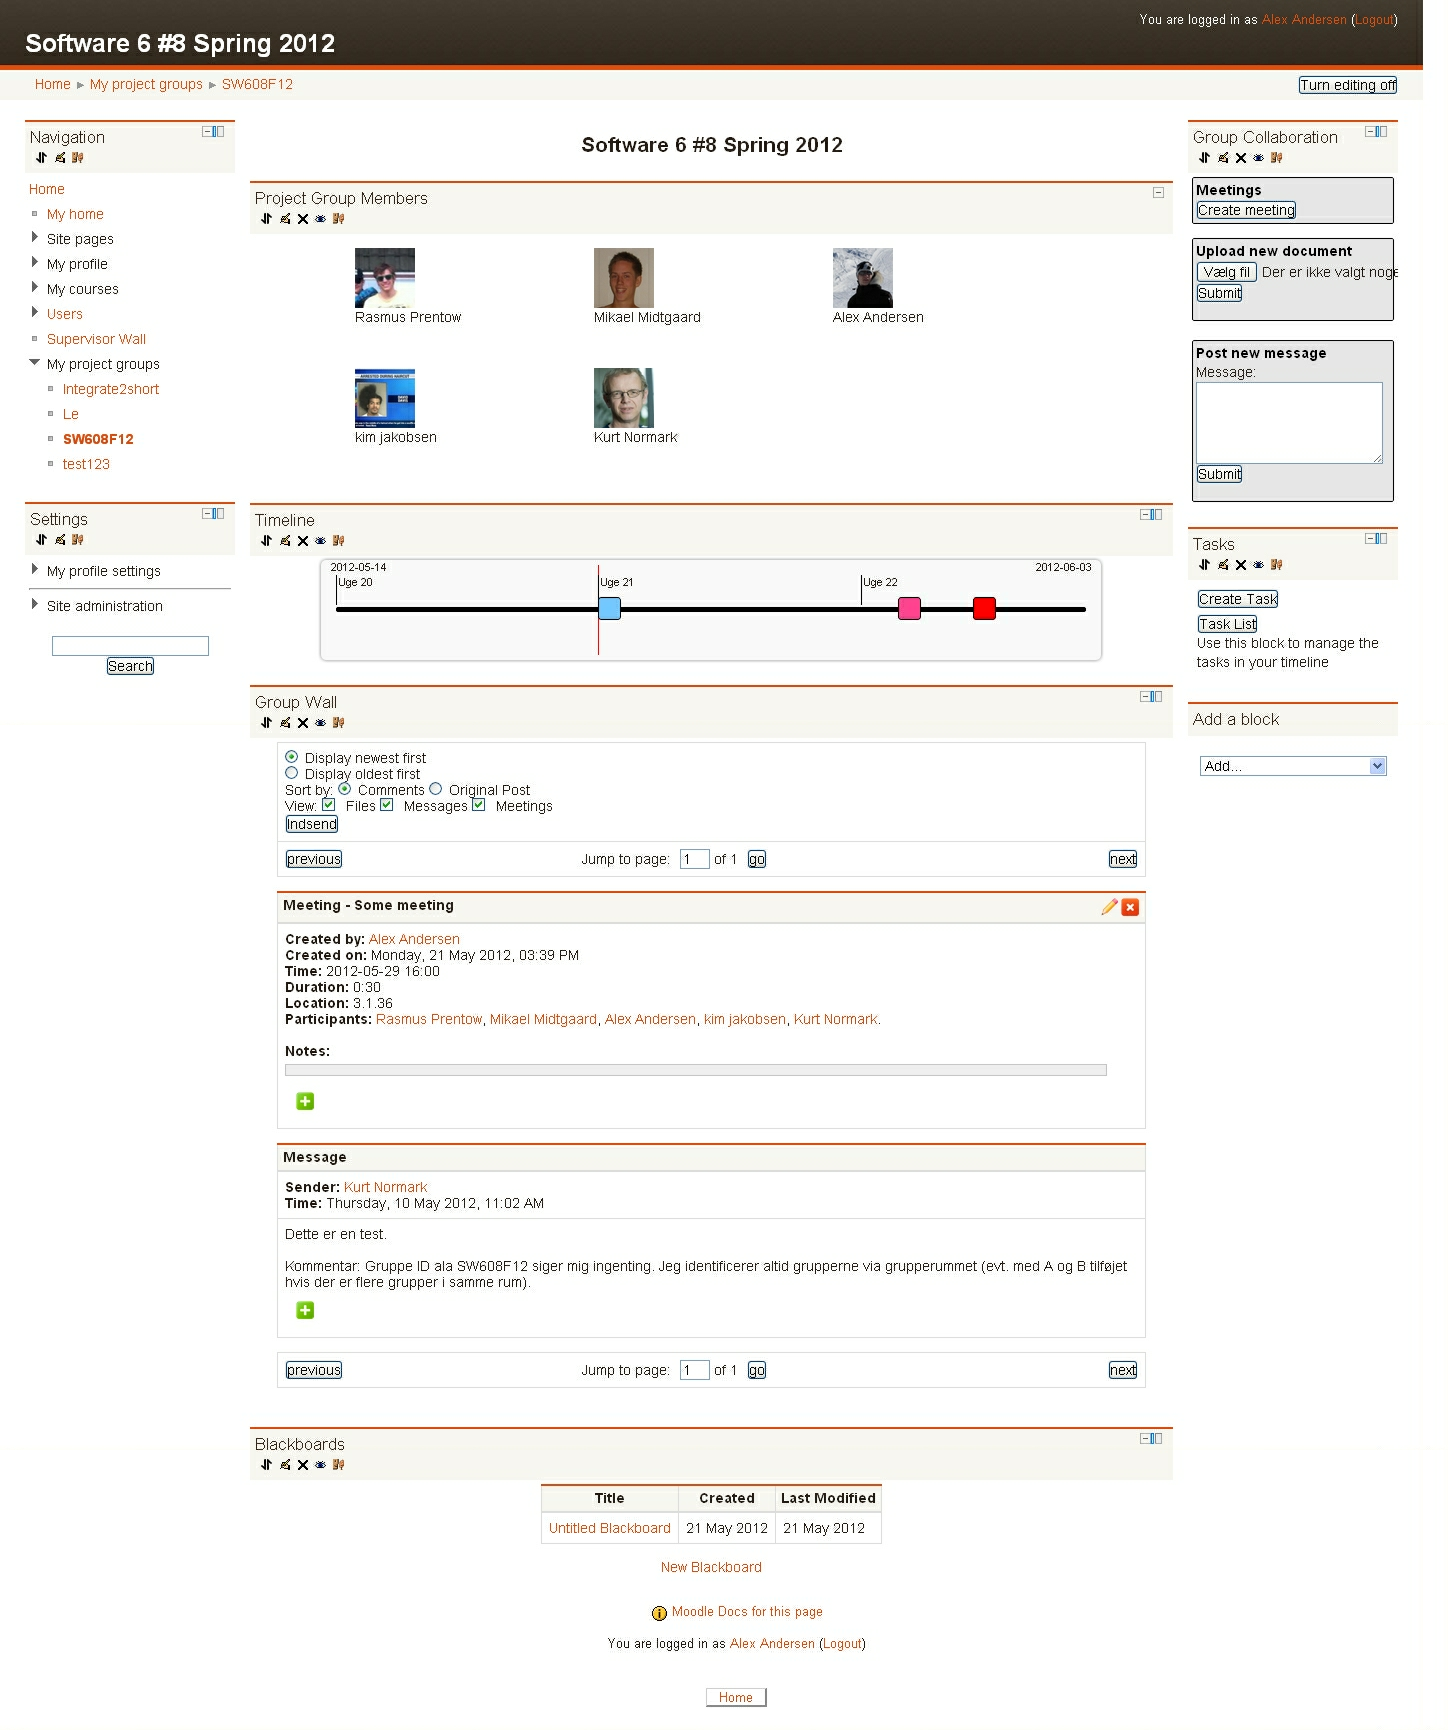
\includegraphics[width=\textwidth]{images/projectgroupwithedit.png}
	\morscaption{The project group room with editing turned on}
	\label{fig:projectgroupwithedit}
\end{figure}


The task of securing that only members of the project group can edit and view are maintained by the project group room and is described in \secref{sec:projectgrouproommanagerights}. 




\subsection{Ensuring Permissions}
\label{sec:projectgrouproommanagerights}
Permissions can generally be divided in two types; read and write. 
Read permissions gives you the ability to view the content of the project group room while write lets you change the content. 
If a user has write permission he must also have read permissions. 
Otherwise he cannot see the page he attempts to edit. 
To ensure the user attempting to enter a project group room has permission to enter the function \fu{has\_projectgroup\_read\_permission} is used. 
It checks if the user is an administrator or is a member of the group. 
The administrator check is necessary since administrators should be able to see the group even if they are not members of the group. 

The function  \fu{has\_projectgroup\_write\_permission} which checks that the user has write permissions uses the read permissions function too check that the user can read.
If he cannot read he should not be able to edit. 
In the current implementation the write permissions function does not make extra checks to permissions since the permission level for read and write is equivalent.
Making both function gives the ability to later change this.
An example could be if the potential users requires that their supervisor should only have read permissions. 
Then the change will be in one place only. 

\subsection{Blocks}
\label{sec:implprojectgroupblocks}
When a new project group is created the default blocks are added to the page. 
The default blocks are specified in the a config file and the content can be seen in \coderef{moodledaultblock}


\begin{lstlisting}[style=phpCode, caption=\myCaption{The default block configuration}, label=moodledaultblock]
<?php
	/**
	* Example usage:
	* "left1,left2:center1:right1"
	* Will add two items to the left, one in the middle, and one to the right
	*/
	$format['defaultprojectgroupblocks'] = ':projectgroup_members,timeline,groupwall,blackboard:upload,tasks';
\end{lstlisting}\begin{comment}$\end{comment}
The syntax for the format is $left:middle:right$. 
Left, middle, and right represent the three columns in the project group room. 
The blocks: Timeline, groupwall, blackboard, upload, and tasks is created by our peer-groups while the block named projectgroup\_members is created by us. 
The projectgroup\_members block shows the name and pictures of the project group members. 

	
	


\subsection{Overwrite Context}
In \secref{sub:contextsystem}  the context system of Moodle is described.
In this section the creation of a custom context is described. 

To be able to define capabilities for the project groups and have different blocks for different project group we need our own context.
We will create our own context level and class.
We call the context \cl{context\_projectgroup}. 

Moodle does not support extension of contexts through one of the more than 30 different plugin types available \cite{plugin}. 
There two parts of the problem, the first is to create a new context and the second is to load it properly. 
We create a new context by making a new class which is very similar to \cl{context\_course} class and by defining the context level of project groups as a constant. 
The class header and the constant definition can be seen in \coderef{codeprojectgroupcontext}. 
The constant is set to 55 and is chosen because that context level is unused and it is close to the course context level. 
We regard the project group contexts to be at the same level as course contexts. 
However, project groups does not have categories like courses does.

\begin{lstlisting}[style=phpCode, caption=\myCaption{The context\_projectgroup class header and constant definition}, label=codeprojectgroupcontext]
define ('CONTEXT_PROJECTGROUP',55);
class context_projectgroup extends context {
...
\end{lstlisting}

When a context is loaded in a Moodle page it is instantiated by \fu{get\_context\_instance}, which takes a context level and an instance id. 
The instance id can be a course id or similar depending on the context level -- in our case it is a project group id. 
This function calls a static method in the \cl{context\_helper} class which uses a private array to translate the context level into a class name.
The overall system definition in \chapref{chap:systemDef} retain us from changing the core code of Moodle. 
If this constraint were not enforced the array could simply be extended directly in the code.  
Since the array used is private we can not extend the context system by overriding the \cl{context\_helper} class. 
The newly created context is only used in pages created in this project and we can therefore create our own version of \fu{get\_context\_instance}. 
The new function can be seen in \coderef{codeprojectgroupcontextinstance}.
\begin{lstlisting}[style=phpCode, caption=\myCaption{The function to get projectgroup context}, label=codeprojectgroupcontextinstance]
function get_projectgroup_context_instance( $instance = 0, $strictness = IGNORE_MISSING) 
{ 
    return context_projectgroup::instance($instance, $strictness);
}
\end{lstlisting}
The \vari{instance} variable denotes a project group id.
The \vari{strictness} variable 

With the new context and the function to instantiate it we can now make per project group permissions and add blocks to specific project group pages. 



\subsection{Navigation}



























\section{Managing Project Groups} %Jeg skriver kun om admin funktionalitet her -Mikael ~♥
Before any project group can be useful it has to be created first.
Administrators need to have the ability to add, edit, and delete project groups.
The administration tools we provide have to be easy and fast to use, since they potentially have to be used many times.
This section describes how we implemented the administration tools needed to manage project groups.

The features we provide to manage project groups are known as administration tools in Moodle and can be accessed in the site administration menu as seen in \figref{fig:navigation}.

\begin{figure}[htb]
	\centering
		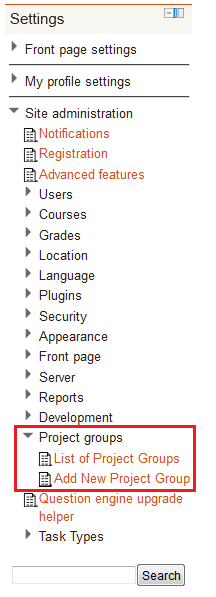
\includegraphics[scale=0.75]{images/admin-navigation.png}
	\morscaption{The settings block, which contains the site administration menu} 
	\label{fig:navigation}
\end{figure}

From here we provide a link to a list of all project groups and a link to a page, from where a new project group can be created.
The page with the list of all project groups has a table with three columns: Short name, Full name, and Actions.
As the name indicates Short name is a short name for a group. 
The Short name also serves as a link to the project group page described in \recref{sub:page}.
In the Actions column there are links to delete and edit the project group.

The edit page has the same source files as the add page.








	
	\chapter{Test}
\label{chap:test}
\myTop{This chapter describes how we perform testing of the code written in this project.
Additionally there is a discussion on how effective the testing is.
Testing is important, since it helps find the bugs in the program and thereby making the end product better.}


\section{Strategy}
\label{sec:strategy}
\newcommand{\idealCC}{$60\%$}
Our development is to some extent test driven.
This means that we are creating unit tests for our functionalities and integration tests to test whether or not our \subsystem{} as a whole work as expected and work together with \moodle{}.
As mentioned in \secref{sub:testing} we are using SimpleTest to test our PHP code.
When we know what a function is supposed to do prior to its implementation we write test cases for the function.
If we do not write test cases prior to its implementation we write test cases for the function after its implementation. 
%Even though it is likely that the person who made the function is the same person as the one who writes the test cases, there are still bugs to be found by this method.
Since working with Moodle is new to us we do not have a full understanding of the Moodle core API.
% which means that in some cases we will expect a function to return something other than what it actually returns.
This means that even with the documentation of the \moodle{} core API we may misinterpret the behavior, input, or output of a function.
Many bugs related to this are discovered by writing test cases.

There is code in this project which is not included in functions and are not included in any unit tests.
This include code belonging to our user interfaces (UI).
%, referred to as views.
These UIs are tested using UI testing, which is conducted by the developer to ensure that the functionality is as expected, and through the demo meetings where the system is tried out. 

The test cases we write do not catch all bugs in the system, but that does not mean that they do not serve a purpose.
Apart from the bugs they actually catch, they also improve the robustness of the system.
If someone decides that the implementation of a function should be altered the test cases can be used for regression testing and thereby reducing the risk of failures. 
This is especially important in our case since a new group of people will continue our work later.

A metric for determining how well some software is tested is code coverage. 
The specific type of coverage we measure our code with is line coverage. 
Determining the percentage of coverage we strive for is a cost/benefit situation.
On one hand we want a stable system that is working as intended, but on the other hand we do not want to spend all our time writing test cases.
The importance of testing is based on the criticality of the system.
The radar chart in \secref{subsec:choosingmethod} shows that if our system fails it will only affect the comfort of the users.
Low criticality calls for a relatively low code coverage.
We choose that \idealCC{} line coverage is sufficient for our core functionality.
Our core functionality being the \admlib{} and project group library.
An evaluation of our testing can be seen in \secref{sec:results}.

In addition to considering code coverage we choose to perform equivalence partition~\cite[pp.~67-69]{Patton05} and boundary value analysis (or data testing)~\cite[pp.~70-79]{Patton05} in the creation of test cases.
Without going into too great details of these concepts, equivalence partitioning means that for every function we test, we partition input values into partitions.
Within these partitions the outcome of each element is expected to be the same.
Consequently we have to test at least one element in each partition, but not necessarily every element.
A boundary value analysis is performed by identifying boundary values and selecting values around each boundary value for testing, e.g. if 0 is a boundary value for some integer input, -1, 0, and 1 is chosen for test values.
Boundary values are identified as values that delimit a boundary, described by \citeauthor{Patton05} to be ``like the edge of a cliff''~\cite[p.~71]{Patton05}.
These can be the value where elements change from being in one partition to being in another.
Alternatively it can be special objects of the certain input type, such as null, empty string, or empty array.
\section{Test Implementation}
\label{sec:testimplementation}

Implementing the testing is done by writing a number of test cases that use the functions and check if they behave as they should.
There is built-in functionality to see how many of the SimpleTest test cases pass.
This tool is used every time a function is implemented, to see if the function corresponds to its expectation.

\begin{lstlisting}[style=phpCode, caption=\myCaption{A test case for the function createTestGroup. The test case tests if the function handles editing of the short and full name correctly.}, label=testcaseedit]
function testEditGroupChangeShortFullName() {
		global $DB;
	  
		//The data
		$projectgroup = new stdClass();
		$projectgroup ->shortname = "EditGroupChangeMembers";
		$projectgroup ->fullname = "EditGroupChangeMembers";
		
		//Create a group
		$groupID1 = $this->createTestGroup($projectgroup);
		
		//Loads the created table from db
		$projectgroupToBeEdited = $DB->get_record($this->groupTableName,array('id'=>$groupID1));
		
		$projectgroupToBeEdited->shortname = "dope is the dope";
		$projectgroupToBeEdited->fullname = "dope is the mope";
    
		//$projectgroupToBeEdited now contains an id property and new members
		$groupID2 = $this->createTestGroup($projectgroupToBeEdited);
		
		$result = $DB->get_record($this->groupTableName,array('id'=>$groupID1));
    
		//It is the ID the same?
		$this->assertEqual($groupID1,$groupID2);
		$this->assertEqual($result->shortname,"dope is the dope");
		$this->assertEqual($result->fullname,"dope is the mope");
}
\end{lstlisting}

In \coderef{testcaseedit} a test case for the function 
\section{Results}
\label{sec:results}

In this section we evaluate the test cases code coverage. 
Moodle has an inbuilt functionality for line coverage of unit tests, which we use to measure the code coverage.

We have to unit test files, one for the project group library and one for the admin tool library. 
And a report is generated for both and can be seen in \appref{app:localcc} and \appref{app:admincc}.
The line coverage for the project group library is $68.09\%$ and $77.06\%$ for the admin tool lirary.

As stated in \secref{sec:strategy} a good line coverage for a production sites code coverage is \idealCC{}.
Our line coverage is above this and considered acceptable for the kind of system we are building. 
Striving to achieve more will not give a cost/beneficial result \todo{cite til testing her}. 
Our tests are combined with several UI tests which helps find bugs and ensure better quality of the product. 


	
	
\part{Evaluation}
	
	
\chapter{Evaluation}

\section{Discussion}

\chapter{Conclusion}
\label{chap:conclusion}
\myTop{In this chapter the project is concluded upon in two ways. Initially we will conclude upon the multi-project, and then we will conclude upon our sub-project.}
\section{Multi-Project}
\label{sec:multiconclusion}
In the first part of this report the system definition for the multi-project, \system{}, is presented as the following: 

%shared system statement
\sharedInput{system_definition}
%MyMoodle is a extension to Moodle that allows Moodle to
%support the Aalborg PBL model. MyMoodle will not interfere
%with other functionalities in Moodle.

The support we wished to provide for the Aalborg PBL model was a virtual group room.
We chose this because a group room is an essential part of working together on a project in the Aalborg PBL model. This system serves as a tool that supports group work for students with a persistent physical group room.
Additionally, it serves as persistent meeting place for students who need to reserve a group room on a daily basis or do not have a physical group room at all.

The services that the virtual group room provide are a virtual blackboard, a tool for communication between students and supervisors, and a time management tool.
The virtual blackboard is a place where creative work and notes can be produced collaboratively by students in a project group and saved for later use.
Communication between students and supervisors is done by writing on a message board and planning meetings.
Each project group has an individual message board and each supervisor has a personal message board displaying messages from every project group that he supervises.
The time management tool allows for arrangement of tasks, and shows these in a simple timeline display.
This timeline also shows blackboard events and planned meetings.

These tools allow students to work in a project group following the Aalborg PBL model through the existing platform \moodle{}.

%These tools allow students to work in a project group following the Aalborg PBL model even when they have no physical group room available.
%To allow a project group to manage the time they have available they can use the 
%allows for creative work and 
%something blackboard timeline supervisor somethingsomething

The virtual group room is implemented as a ``local plugin''.
The content of the virtual group room is \block{}s.
These contain the tools described above or have links to the functionalities of the tools.
Since every component of \system{} is implemented as a \moodle{} plugin we have not changed anything in the core code of \moodle{}.
This ensures that we do not change other functionalities in \moodle{}.
Thereby \system{} is an extension to \moodle{} that supports the Aalborg PBL model as defined in the system definition.

\section{Sub-Project}
\label{sec:subconclusion}

In the second part we defined the sub-system we, as four people, developed during this project.
The system was defined as:

%our system statement
\begin{center}
\framebox[0.85\textwidth][c]{
	\parbox{0.8\textwidth}{
		\textsl{A \subsystem{} of \system{} that implements project groups in Moodle and allow for administration and usage thereof. 
			The \subsystem{} includes a virtual meeting place, which integrates the other subsystems. 
		}
	}
}
\end{center}
%A sub-system of MyMoodle that implements project groups in
%Moodle and allow for administration and usage thereof. The
%sub-system includes a virtual meeting place, which integrates
%the other subsystems

We implemented an administration tool in accordance with Moodle standards.
By using this tool administrators are able to add, edit, and delete project groups.
In order to accommodate for a large number of project groups we have created a page with a list of all project groups.
Finding a specific project group or a specific set of project groups is possible by using filtering.

Additionally, we created a project group room page based on requirements gathered from interviews and demo meetings conducted during the project.
Each project group has one of such pages associated with it.
This page shows all the group members with name and profile picture, and allows other \system{} blocks to be displayed.

To allow integration between the \subsystem{}s of \system{} we provide a code library that is available in every \moodle{} page.
This library has data retrieval functions to project groups.
These include retrieval of project groups related to a specific user and retrieval of project group information (name, members, etc.) of a specific project group.
For our administrative tool we have created a separate library.
Our libraries are documented and tested to an acceptable extend for the kind of system we have developed.

The structure of our system allows for further development in a modular fashion.
It also allows for changes in the implementation while keeping the system robust.
%Together this provides a system that can be extended further by the students next year. 
%indefinitely












\section{Perspective}



	
		
		%\subsection{Moodle Context System}
		%A major part of moodle is the context system which is in charge of bo
		
		
		

	%Bibliography
	\cleardoublepage
\addcontentsline{toc}{chapter}{\numberline{}Bibliography}
\label{chap:bib}
\bibliography{bib,\sharedReport bib}
\listoffigures
\lstlistoflistings

\appendix	
	\part*{Appendix}

\chapter{Interviews}

\section{Lene Winther Even}
\label{sec:lene}
Interviewers: Kim A. Jacobsen and Mikael Midtgaard\\


This interview was conducted on March 15\ths{} at Cassiopeia at Aablorg University.
At the time of writing Lene is a Senior Secretary at Aalborg University, and one of her tasks is to handle many aspects of Moodle for the Institute of Computer Science.

The following is a transcript of the interview.

\subsection*{Moodle in General}
It is a problem that there are 13 different Moodle systems at Aalborg University, especially since some student are required to use more than one Moodle system.

When there is a change in a calender event it is difficult to administer in Moodle.

Only students, administrative personnel, teachers, supervisors use Moodle.
Research groups currently do not use Moodle to share information.




\subsection*{Project Groups}
Project groups are created manually by writing them in a course.
Currently the university view groups and projects as one.
Messages for project groups are sent by email.
This could be improved by sending the messages through Moodle.
Messages to entire semesters are sent through Moodle.
A forum can be created for each project group to be used for a group's internal and supervisor communication.
The implementation in Moodle version 1.9 by default sends emails to the whole semester.




\subsection*{Other Tools}
Lene could tell us of some of the other tools that were used in relation to the Moodle system.

\subsubsection*{ADMDB}
ADMDB is the Administration Database and is maintained by the Information Services Technology department(IST).
The database is not currently linked with Moodle; all information from the database has to be written manually into the Moodle system.
The database was linked with the old TYPO3 system.
We learned more about ADMDB from SOMEGUY ALSO MAKE REF. \todo{ref to other interview}

\subsubsection*{CalMoodle}
CalMoodle is a calender system for courses.
Calender events are created in CalMoodle and imported to the Moodle system.
Calender events have no direct relation to courses.

\subsubsection*{Office}
Different programs from the Microsoft Office suite are used to store and manage data locally.




\subsection*{Courses}
Some courses at Aalborg University share some of the same information.
However, that information has to be written to the courses individually.
It is highly wanted for courses to share some common information.

Administrative personnel are enrolled to a many courses, which all are listed on the front page and in the navigation menu.
This clutters the main page as well as making navigating to a specific course difficult.

School of Information and Communication Technology(SICT) are responsible for creating a Moodle course for each course as well as a Moodle course for each semester. 
Students are automatically assigned to the semester course.
The administrative personnel write some general information to the courses.
Additional information are written by the lecturer.
Course information is often copied and pasted different places.

Students are automatically added to the semester course, but they have to manually enroll to every other course.
Teachers are added to courses with the role of a student, and an administrator has to manually promote them.




\subsection*{Archiving}
Finished reports are the only thing that is currently being archived.
They are archived in the project database.
Supervisor contact and meetings are relevant candidates for being archived.
ELSA have plans for archiving all courses and course information for future reference.
\end{document}
